%File: supplementary_v14.tex --- Technical Appendix (AAAI-27 anonymous submission, final; includes Section L: scale and external-map studies)
\documentclass[letterpaper]{article} % DO NOT CHANGE THIS
\usepackage[submission]{aaai2027}  % DO NOT CHANGE THIS
\usepackage[hyphens]{url}  % DO NOT CHANGE THIS
\usepackage{graphicx} % DO NOT CHANGE THIS
\urlstyle{rm} % DO NOT CHANGE THIS
\def\UrlFont{\rm}  % DO NOT CHANGE THIS
\usepackage{natbib}  % DO NOT CHANGE THIS AND DO NOT ADD ANY OPTIONS TO IT
\usepackage{caption} % DO NOT CHANGE THIS AND DO NOT ADD ANY OPTIONS TO IT
\frenchspacing  % DO NOT CHANGE THIS
\usepackage{booktabs}
\usepackage{amsmath}
\usepackage{needspace}
\pdfinfo{
/TemplateVersion (2027.1)
}
\setcounter{secnumdepth}{0}

% Float packing: this appendix is table-dense; allow more floats per page so
% tables land near the sections that introduce them.
\setcounter{topnumber}{3}
\setcounter{totalnumber}{5}
\renewcommand{\topfraction}{0.88}
\renewcommand{\textfraction}{0.1}
\renewcommand{\floatpagefraction}{0.8}

\newcommand{\stage}[1]{\textsc{#1}}

\title{Technical Appendix: An Empirical Analysis of Transfer for Dynamic Path Planning}
\author{Anonymous Submission}
\affiliations{}

\begin{document}
\maketitle

This appendix is organized by claim: protocol and implementation specifications (A--B), the dynamic zero-shot result with its replications, classical controls, and audit trail (C), adaptation and the matched-label factorial (D), boundary experiments (E--H), validity forensics (I), statistics and the map-clustered reanalysis (J), reproducibility (K), and the scale and external-map studies (L).

\section{A. Protocols by Stage}

All continuous stages share the substrate: a 2-D point robot, maps with procedurally generated obstacles, a probabilistic roadmap (PRM) of exactly 192 nodes with $k{=}7$ connectivity, and A\textsuperscript{*} evaluated at a per-suite \emph{binding budget} of node expansions. Budgets are calibrated on the anchor baseline only, toward pre-specified target success rates. The exact grid, selection rule, and realized rates are in Table~\ref{tab:calib}. Per-stage protocol essentials are summarized in Table~\ref{tab:protocols}. Unless noted, training labels are exact graph-Dijkstra costs on the PRM (static) or exact backward space--time Dijkstra values over $(\text{node},t)$ (dynamic). Headline continuous runs are local single-GPU (RTX 5090) validations with one primary training seed unless stated. The discrete program ran on a remote fleet.

\section{B. Environment, Model, and Data Specifications}

\begin{table*}[t]
\centering
\small
\begin{tabular}{@{}lp{14.2cm}@{}}
\toprule
Stage & Protocol essentials \\
\midrule
\stage{C1--C4} & 9 easy suites, $n{=}80$/40 maps, budgets 100--200; pooled bases, TaskLoRA experts, RBF mixtures. \\
\stage{C5} & calibrated hard maze/dense/rooms; 160 train maps; 80 eval maps attempted per suite, 80/79/77 retained after world-build filters; budgets 128--168; scalar residual target with cap. \\
\stage{C6} & goal-conditioned raster residual field (8 input channels), sampled at PRM nodes; 96/40 maps; budgets 128--168. \\
\stage{C7} & 6 suites (3 held out: one distinct topology, two shifted variants); 96/24 maps per suite; binding budgets 140 (maze/dense/rooms/spiral), 24 (bugtrap), 56 (rooms-large); scalar+field $\times$ additive+focal matrix; exact-Dijkstra oracle. \\
\stage{C8} & deterministic moving circular obstacles; space--time PRM; aware ($W{=}8$ future window) vs.\ blind ($W{=}0$) twins; canonical run: 53 usable training worlds (maze/rooms/spiral; collection details and exact label counts in Section~B); 20-map/suite \emph{development} cohort, then a 50-map/suite \emph{confirmation} cohort evaluated after freezing, plus two independent full-pipeline retrains (139/149 worlds) on the same confirmation cohort. \\
\stage{C9/C9h} & adapt \stage{C7} pooled bases to the 3 held-out targets; $K \in \{0, 1, 2, 4, 8, 16, 32\}$ labeled maps; LoRA(r8, bounded/unbounded), full FT, scratch; \stage{C9h} matches compute (10 epochs, LR $2{\times}10^{-4}$); 30 fixed test maps/target. \\
\stage{C9b} & same protocol on \stage{C8} dynamic sources (aware+blind), 486 adapters, 3 targets, $K\in\{1,4,16\}$. \\
\stage{C10} & 16 rank-8 experts on 2 family axes; zero-label transfer to 3 interior targets; RBF/nearest/uniform weight-merge and prediction-mix composition. \\
\stage{C11} & compositional missions (waypoint sequences; key/door), configs A/B/C, mission length $K\in\{0,2,4,8\}$; 40 train / 25 test maps per cell; 6 learned arms $\times$ 3 seeds (198 checkpoints; 54{,}450 eval rows); exact mission oracle and leg-sum baseline; forced-compute and would-halt probes. \\
\stage{C12} & (A) hidden slow/fast regime dynamics, memory-headroom gate, matched temporal-hierarchy pilot; (B) tied vs.\ untied product-graph refiner, cycles 1--8, configs A/C $\times$ $K\in\{2,8\}$, 3 seeds, 48 checkpoints, two 3{,}200-row test tables. \\
\stage{C13} & current-state heuristic under bounded observation (radius 0.20 local subgraph); behavior-derived fresh-start rollout labels (median of 3); staged falsification ladder (\stage{A}--\stage{L}) then frozen 144-map confirmation (\stage{M}); architecture substitutions (\stage{N}/\stage{O}); persistent-state pilot (\stage{P}). \\
Discrete & 20$\times$20 to 256$\times$256 grids; Manhattan-baseline A\textsuperscript{*}; forecasting (dynamic obstacles), additive residual transfer (22 suites $\times$ 3 budgets $\times$ 100 episodes), pooled multitask bases, learned focal ranking at $w\in\{1.0,1.05,1.1\}$. \\
\bottomrule
\end{tabular}
\caption{Protocol essentials by stage: substrate, cohorts, budgets, and supervision, abbreviating the full specifications in Sections~A--B and each stage's own section; stage labels match the main paper.}
\label{tab:protocols}
\end{table*}

\textbf{World generation.} Continuous worlds are square (side length 1.0; 2.0 for the large-room family); units are abstract. Start and goal are sampled with minimum separation 0.45 of the side length. Each roadmap has 192 nodes in total (the start and goal at indices 0 and 1 plus 190 sampled free-space nodes), with $k{=}7$ nearest-neighbor candidate edges per node (doubled for the start and goal, then symmetrized). Edges are validated by collision sampling at resolution 0.010 of the side length, and worlds whose roadmap fails to connect start to goal are rejected and resampled. Table~\ref{tab:envspec} gives the per-family generator rules, Table~\ref{tab:dynspec} the dynamic-obstacle specifications, and Table~\ref{tab:archspec} the instantiated architectures with exact parameter counts.

\begin{table}[t]
\centering
\small
\setlength{\tabcolsep}{2.5pt}
\begin{tabular}{@{}lp{5.6cm}@{}}
\toprule
Family & Generator rule (lengths as fractions of side length) \\
\midrule
Maze / dense maze & Corridor maze of axis-aligned walls; the dense variant narrows gap width to 0.115. Held out: dense. \\
Rooms / large rooms & $2{\times}2$ rooms from one vertical + one horizontal partition wall, one doorway per wall, doorways biased toward opposite edges; large variant doubles side length. Held out: large. \\
Spiral & Four serpentine vertical walls spanning $x \in [0.22, 0.78]$, gap side alternating per wall. Trained. \\
Bugtrap & Solid vertical back wall, two horizontal arms, and a mouth lip closing the center of the opening (U-pocket). Held out. \\
Crossing (dyn.) & Open arena; dynamic timing control. \\
\bottomrule
\end{tabular}
\caption{Static geometry per family. The base families of the early stages (the nine easy open/clutter/narrow suites of \stage{C1}--\stage{C4}) also place 3--68 circular obstacles with radii 0.022--0.115; full ranges ship with the generator in the artifact package.}
\label{tab:envspec}
\end{table}

\begin{table}[t]
\centering
\small
\setlength{\tabcolsep}{2.5pt}
\begin{tabular}{@{}lcccccc@{}}
\toprule
Suite & Patr. & Radius & Span & Period & $v_{\mathrm{ag}}$ & $t_{\max}$ \\
\midrule
Maze & 3 & 0.075 & 0.38 & 0.14 & 0.060 & 110 \\
Rooms & 3 & 0.075 & 0.40 & 0.14 & 0.060 & 110 \\
Spiral & 3 & 0.075 & 0.38 & 0.14 & 0.060 & 110 \\
Dense maze & 4 & 0.062 & 0.42 & 0.17 & 0.060 & 140 \\
Crossing & 4 & 0.055 & 0.50 & 0.30 & 0.060 & 110 \\
Large rooms & 5 & 0.075 & 0.36 & 0.14 & 0.120 & 130 \\
\bottomrule
\end{tabular}
\caption{Dynamic-suite parameters. Each patroller is a circle sweeping a line segment with triangle-wave motion. Radius and span are fractions of the side length, period is a fraction of the horizon $t_{\max}\,dt$ ($dt{=}1$\,s), and each patroller crosses its span twice per period. Sweep centers carry lateral jitter $\leq 0.02$ (0.10 on crossing). The planner and collision checker always use these exact trajectories. Only the \emph{aware} heuristic input sees the $W{=}8$ future-occupancy channels.}
\label{tab:dynspec}
\end{table}

\begin{table*}[t]
\centering
\small
\setlength{\tabcolsep}{1.6pt}
\begin{tabular}{@{}lccc@{}}
\toprule
Model & Configuration & Input & Parameters \\
\midrule
Scalar HRM & hid.\ 192, 2 layers, 4 heads, $k{=}2$ & 62 tok.\ $\times$ 16 & 2{,}158{,}529 \\
Scalar ON-LSTM & hid.\ 256, 2 layers, chunk 8 & 62 tok.\ $\times$ 16 & 1{,}252{,}481 \\
Field U-Net & FiLM-cond.; base 32, enc.\ 32-256 & $64{\times}64$ raster & 3{,}702{,}370 \\
Field HRM & conv stem /4; hid.\ 256, 2 lay. & $64{\times}64$ raster & 4{,}016{,}642 \\
Field ON-LSTM & conv stem /4; hid.\ 256, chunk 8 & $64{\times}64$ raster & 1{,}448{,}578 \\
\midrule
Mission MLP & 3 GELU layers, width 768 & mission tok. & 1{,}274{,}881 \\
Mission U-Net & FiLM stage emb.\ (32) at bottleneck & raster+stage & 2{,}096{,}521 \\
Mission GNN & hid.\ 128, 8 untied rounds & graph & 681{,}089 \\
Mission HRM-tr. & hid.\ 224, $k{=}2$, 4 heads, head 256 & mission tok. & 2{,}901{,}473 \\
Mission ON-L.-tr. & hid.\ 256, chunk 8, head 256 & mission tok. & 1{,}251{,}457 \\
Mission HRM-v2 ACT & forced-$k$ port of HRM-tr. & mission tok. & 3{,}414{,}786 \\
Big U-Net / HRM & base 64 / hid.\ 512 (addendum) & as above & 14{,}824{,}161 / 15{,}015{,}937 \\
\bottomrule
\end{tabular}
\caption{Primary instantiated architectures with parameter counts computed from the released constructors (mission arms are constructor-verified to lie in the preregistered $[0.5\mathrm{M}, 3.5\mathrm{M}]$ band; the test suite asserts the counts; the early-stage scalar MLP/LSTM baselines are in the artifact archive). Scalar token sequences: one summary token, 12 nearest-obstacle tokens, 48 ray tokens, one goal token. Dynamic variants append $W$ future-occupancy channels ($W{=}8$ aware; $W{=}0$ blind; the aware U-Net's wider first layer brings it to 3{,}704{,}674 parameters); future frames are rendered from the exact trajectories at real times $(t{+}i)\,dt$, $i \le W$, which are defined for all $t$, so frames beyond the search horizon need no clamping or padding. LoRA \citep{hu2021lora} inserts rank-8 adapters on the HRM (rank-24 on the ON-LSTM, matching its wider hidden layer); the quoted crossover cells are HRM (rank 8); the factorial's dynamic arm applies rank-8 conv-LoRA to every U-Net Conv2d (192{,}080 trainable parameters). Optimizer for all models: AdamW, learning rate $2{\times}10^{-4}$ ($1.5{\times}10^{-4}$ for adapters), weight decay $10^{-4}$, batch 256, gradient clip 1.0, smooth-L1 loss on the capped residual (cap 4.0), 10 base epochs (8 adapter epochs) unless a stage states otherwise. Remaining constructor details (activations, normalization, heads) ship with the code in the artifact archive.}
\label{tab:archspec}
\end{table*}

\textbf{Temporal collision validation.} A wait at node $v$ from step $t$ is valid iff the node position is free over the continuous interval $[t\,dt, (t{+}1)\,dt]$, checked at 8 uniform time samples. Traversing edge $e$ (duration $\tau(e)$ steps) is valid iff sampled points along the edge are free at their interpolated times, with $\max(8, 4\tau(e))$ samples. Arriving at a node (pass-through) requires no additional node check beyond the edge validation. The planner and collision checker always use the exact deterministic trajectories. These sample counts define the implementation's numerical collision predicate. They are not a certified continuous-time check, and every optimality statement, including SIPP's \citep{phillips2011sipp}, is exact with respect to this discretized predicate.

\textbf{Dynamic data collection.} A candidate training world is \emph{usable} iff (i) the world builds, (ii) its roadmap connects start to goal, and (iii) the space--time problem is solvable from the start at $t{=}0$ (finite backward space--time Dijkstra value). Training worlds are drawn only from the dynamic maze, rooms, and spiral families. Collection draws a fixed number of candidate worlds per family from a deterministic per-(family, index) seed stream and keeps the usable ones. The canonical run drew 24 per family and kept 53 (maze 17 / rooms 19 / spiral 17). The seed-2001 and seed-2002 retrains drew 64 per family and kept 139 (41/50/48) and 149 (40/54/55); the collection-budget divergence is disclosed in Section~C. Every usable world has exactly 192 nodes and $t_{\max}{=}110$, i.e.\ 21{,}312 node--time slots. The training loss is masked to states with finite backward space--time values. Exact supervised-label counts from the deterministic recount (which reproduces each run's per-suite world counts as a correctness gate): canonical 821{,}850 of 1{,}129{,}536 slots (72.8\%; per-world mean 15{,}507, range 13{,}028--17{,}322); seed 2001, 2{,}115{,}331 of 2{,}962{,}368 (71.4\%); seed 2002, 2{,}257{,}512 of 3{,}175{,}488 (71.1\%). The reachable fraction is family-dependent (the maze-dense target worlds of the factorial average $\sim$18{,}900 usable states per world).

\begin{table}[t]
\centering
\small
\setlength{\tabcolsep}{2.6pt}
\begin{tabular}{@{}lcccc@{}}
\toprule
Suite & Band (binding) & A@cal.\ & O@cal.\ & A@conf.\ \\
\midrule
Crossing & 150/250 & 0.30 & 1.00 & 0.12 \\
Maze & 1800/2500 & 0.30 & 1.00 & 0.12 \\
Dense maze & 2500/3500 & 0.05 & 0.95 & 0.06 \\
Rooms & 1300/1800 & 0.30 & 1.00 & 0.42 \\
Large rooms & 600/900 & 0.75 & 1.00 & 0.82 \\
Spiral & 2500/3500 & 0.20 & 0.95 & 0.16 \\
\bottomrule
\end{tabular}
\caption{Dynamic budget calibration. Grid: $\{150, 250, 400, 600, 900, 1300, 1800, 2500, 3500\}$ expansions. Rule: for each of two targets evenly spaced in $[0.45, 0.70]$, pick the grid budget with the closest anchor success on the 20 calibration worlds (the development cohort; ties smaller); the smaller selected budget is \emph{binding} (listed first). A@cal./O@cal.: anchor/oracle success at binding on the calibration worlds; the coarse grid can land outside the target band (dense maze has no point near 0.45). A@conf.: anchor success on the 50-map confirmation cohort (cohort drift). Static \stage{C5}--\stage{C6} use the same rule class on their own grids (binding 128--168; realized 0.25--0.62); \stage{C7} budgets are in Table~\ref{tab:protocols}.}
\label{tab:calib}
\end{table}

\clearpage
\section{C. Zero-Shot Transfer: Tables, Replications, Weighted A\textsuperscript{*}, and Audit Trail}

Table~\ref{tab:c7} gives the complete per-suite \stage{C7} static results summarized in the main paper; Table~\ref{tab:c8fixed} gives the \stage{C8} fixed-provider primary view, Table~\ref{tab:c8fresh} the fresh-cohort confirmation, and Table~\ref{tab:c8seeds} the retrain replications. Table~\ref{tab:c8} is a separate post-hoc best-arm view.

\textbf{Multi-seed replication detail (Table~\ref{tab:c8seeds}).} Two full-pipeline retrains (collect + train, seeds 2001/2002) of the aware/blind field U-Net twins were run under a design frozen before training, then evaluated on the same frozen fresh cohort with the canonical binding budgets. \emph{Disclosed protocol divergence:} the replication design specified collection ``identical to canonical'' but set 64 candidate worlds per family, whereas the canonical run had used 24. The retrains therefore trained on 139 and 149 usable worlds versus the canonical 53 (per-family counts in Section~B). The success replication is thus a replication under independent seeds \emph{and} a larger training collection. The two retrains are collection-matched with each other. This divergence was discovered post hoc during the label-count audit and is reported rather than repaired. Matched-ratio medians across seeds: maze 0.047--0.059, rooms 0.117--0.135, spiral 0.065--0.092 (seed-stable); crossing 0.273--0.434, dense maze 0.216--0.625, large rooms 0.250--0.548 (seed-variable).

Preregistered readouts: R1 (success CI excludes zero in $\geq$5/6 suites) 5/6 and 6/6 (pass); R2 (deltas within $\pm 0.15$ of canonical in $\geq$5 suites) 5/6 and 6/6 (pass); R3 (no suite significantly aware-over-blind) fails as stated for seed 2001 (large rooms $+0.080$ $[+0.020,+0.160]$), the same suite whose interval favors the \emph{blind} twin under seed 1234 ($-0.200$ $[-0.320,-0.100]$). Across the 18 seed--suite twin contrasts: 2 intervals exclude zero for aware, 2 for blind, 14 include zero; no suite's interval excludes zero in the same direction under more than one seed (large rooms flips direction between seeds 1234 and 2001). The per-suite future-window effects flip sign across seeds and are consistent with training-seed noise. No retraining, reselection, or recalibration occurred in response to any readout.

\textbf{Matched path quality vs.\ the anchor.} Table~\ref{tab:pathq} reports mean arrival over optimal arrival on the maps jointly solved by the fixed provider and the anchor. Because the admissible anchor's solved arrivals equal the backward space--time optimum on every map (verified across all suites), the learned column is the entire paired difference. The analysis script ships in the artifact package.

\textbf{Success as a function of budget (Figure~\ref{fig:budgetcurves}).} A single evaluation pass at $4\times$ the binding budget on the same frozen cohort yields \emph{exact} success-vs-budget curves for every lower budget (design frozen before launch). The space--time A\textsuperscript{*} expansion order is budget-independent, and a map is solved at budget $B$ iff its recorded solve expansions are $\leq B$. The curves are therefore derived by thresholding, with no re-runs and no interpolation. As a determinism cross-check, thresholding at the binding budget reproduces every fresh-cohort success value exactly (all suites, all providers). The headline result is not an artifact of the calibrated operating point. Euclidean search needs 1.7--2.8$\times$ the binding budget to reach the fixed blind provider's binding-budget success (crossing 2.49$\times$, maze 2.29$\times$, dense maze 1.95$\times$, rooms 1.73$\times$, large rooms 1.94$\times$, spiral 2.80$\times$). By $4\times$ the binding budget every provider converges to the same feasibility ceiling (0.94--1.00); on dense maze the 0.94 ceiling binds even the oracle, reflecting maps unsolvable within the time horizon, and unbudgeted SIPP confirms these ceilings independently: its per-suite success equals them exactly (Table~\ref{tab:sipp}).

\begin{figure*}[t]
\centering
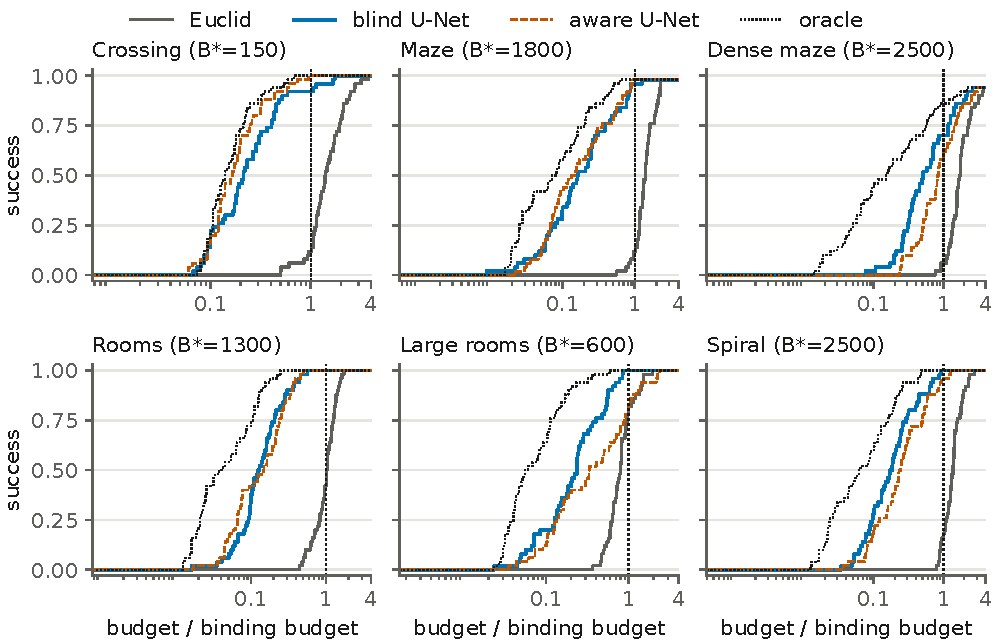
\includegraphics[width=0.98\textwidth]{figures/fig_budget_curves.pdf}
\caption{Success-vs-budget step curves per dynamic suite (fresh 50-map cohort), derived exactly from one $4\times$-binding evaluation pass. Budgets are normalized by the binding budget $B^{*}$ (dashed vertical line). The learned providers reach high success at 0.05--0.3$\times$ $B^{*}$; Euclid requires 1.7--2.8$\times$ $B^{*}$ to match the blind provider's binding-budget success.}
\label{fig:budgetcurves}
\end{figure*}

\begin{table}[t]
\centering
\footnotesize
\setlength{\tabcolsep}{2.2pt}
\begin{tabular}{@{}lccc@{}}
\toprule
Suite & Euclid succ. & Field-HRM succ. & Ratio [95\% CI] \\
\midrule
Maze & 0.583 & 1.000 & 0.521 [0.450, 0.627] \\
Maze-dense & 0.250 & 0.958 & 0.804 [0.707, 0.829] \\
Rooms & 0.375 & 0.958 & 0.829 [0.775, 0.885] \\
Spiral & 0.250 & 0.917 & 0.850 [0.742, 0.919] \\
Bugtrap & 0.458 & 0.750 & 0.714 [0.533, 0.800] \\
Rooms-large & 0.417 & 0.750 & 0.839 [0.646, 1.222] \\
\bottomrule
\end{tabular}
\caption{\stage{C7} static suites at binding budgets: success and matched-solved median expansion ratio (field HRM vs.\ Euclid). Success gains are BH-significant in 4/6 suites (maze, dense, rooms, spiral); bugtrap and rooms-large reach corrected significance only for other learned arms. Scalar-HRM ratios span 0.427--0.822. Matched $n$ ranges 6--14.}
\label{tab:c7}
\end{table}

\begin{table}[t]
\centering
\small
\setlength{\tabcolsep}{3pt}
\begin{tabular}{@{}lcccc@{}}
\toprule
Suite & Euclid & Blind U-Net & Ratio [95\% CI] & $n$ \\
\midrule
Crossing & 0.30 & 0.95 & 0.191 [0.166, 0.878] & 6 \\
Maze & 0.30 & 1.00 & 0.093 [0.057, 0.137] & 6 \\
Dense maze & 0.05 & 0.75 & 0.246 (descriptive) & 1 \\
Rooms & 0.30 & 1.00 & 0.099 [0.050, 0.214] & 6 \\
Large rooms & 0.75 & 0.95 & 0.228 [0.185, 0.418] & 15 \\
Spiral & 0.20 & 0.95 & 0.087 [0.061, 0.287] & 4 \\
\bottomrule
\end{tabular}
\caption{\stage{C8} fixed-provider result on the \emph{original} 20-map development cohort, the calibration worlds (field U-Net blind; no future-motion input; additive mode; binding budgets; map-level bootstraps). Columns 2--3: success. Success deltas are $+0.20$ to $+0.75$ with all six paired CIs excluding zero.}
\label{tab:c8fixed}
\end{table}

\begin{table}[t]
\centering
\small
\setlength{\tabcolsep}{3pt}
\begin{tabular}{@{}lcccc@{}}
\toprule
Suite & Euclid & Blind U-Net & Ratio [95\% CI] & $n$ \\
\midrule
Crossing & 0.12 & 0.92 & 0.273 [0.109, 0.516] & 6 \\
Maze & 0.12 & 0.96 & 0.047 [0.021, 0.153] & 6 \\
Dense maze & 0.06 & 0.70 & 0.216 [0.100, 0.281] & 3 \\
Rooms & 0.42 & 1.00 & 0.121 [0.106, 0.172] & 21 \\
Large rooms & 0.82 & 1.00 & 0.250 [0.188, 0.306] & 41 \\
Spiral & 0.16 & 1.00 & 0.092 [0.065, 0.146] & 8 \\
\bottomrule
\end{tabular}
\caption{\stage{C8} fixed-provider \emph{replication} on the fresh 50-map-per-suite cohort (generation seed 999999, frozen before any result was observed; map-disjoint from the original cohort by the evaluation seed formula's within-suite offset bound). Success deltas are $+0.18$ to $+0.84$ with all six paired CIs excluding zero. Map-paired aware$-$blind success deltas on this cohort: crossing $+0.080$ $[+0.020,+0.160]$, maze $+0.020$ $[0.000,+0.060]$, dense maze $-0.120$ $[-0.220,-0.040]$, rooms $0.000$, large rooms $-0.200$ $[-0.320,-0.100]$, spiral $-0.040$ $[-0.100,0.000]$: one suite's interval favors the aware twin, two the blind twin, three neither.}
\label{tab:c8fresh}
\end{table}

\begin{table}[t]
\centering
\small
\begin{tabular}{@{}lrrr@{}}
\toprule
Suite & $n$ & Subopt. & Paired diff [95\% CI] \\
\midrule
Crossing & 6 & 1.216 & $+0.216$ $[+0.107,+0.382]$ \\
Maze & 6 & 1.004 & $+0.004$ $[+0.000,+0.013]$ \\
Dense maze & 3 & 1.000 & $+0.000$ $[+0.000,+0.000]$ \\
Rooms & 21 & 1.031 & $+0.031$ $[+0.014,+0.051]$ \\
Large rooms & 41 & 1.095 & $+0.095$ $[+0.071,+0.121]$ \\
Spiral & 8 & 1.027 & $+0.027$ $[+0.010,+0.046]$ \\
\bottomrule
\end{tabular}
\caption{Matched path quality versus the anchor on the fresh confirmation cohort: mean learned arrival over optimal arrival on the $n$ maps solved by both the fixed blind U-Net and the anchor at binding budgets. The anchor's arrivals equal the optimum on every anchor-solved map in every suite (admissible heuristic; verified from the raw rows), so the paired learned$-$anchor difference equals the learned excess (10k map-bootstrap CIs). The additive heuristic pays its largest premium on crossing. Dense maze's three joint maps are solved optimally.}
\label{tab:pathq}
\end{table}

\begin{table*}[t]
\centering
\small
\setlength{\tabcolsep}{2.6pt}
\begin{tabular}{@{}lccc@{}}
\toprule
Suite & Seed 1234 & Seed 2001 & Seed 2002 \\
\midrule
Crossing & $+0.80$ [0.68, 0.90] & $+0.86$ [0.74, 0.96] & $+0.88$ [0.78, 0.96] \\
Maze & $+0.84$ [0.74, 0.94] & $+0.86$ [0.76, 0.96] & $+0.84$ [0.74, 0.94] \\
Dense maze & $+0.64$ [0.50, 0.78] & $+0.46$ [0.32, 0.60] & $+0.56$ [0.42, 0.70] \\
Rooms & $+0.58$ [0.44, 0.72] & $+0.58$ [0.44, 0.72] & $+0.58$ [0.44, 0.72] \\
Large rooms & $+0.18$ [0.08, 0.30] & $+0.10$ [$-$0.02, 0.22] & $+0.16$ [0.06, 0.26] \\
Spiral & $+0.84$ [0.74, 0.94] & $+0.84$ [0.74, 0.94] & $+0.84$ [0.74, 0.94] \\
\bottomrule
\end{tabular}
\caption{\stage{C8} preregistered multi-pipeline replication: paired success deltas (blind U-Net $-$ Euclid, map-level 95\% CIs) for three independently trained pipelines on the same frozen fresh cohort (the retrains used larger training collections; see the multi-seed detail paragraph). 17 of 18 CIs exclude zero. The one interval that includes zero is seed 2001's near-ceiling large-rooms cell (Euclid 0.82).}
\label{tab:c8seeds}
\end{table*}

\begin{table}[t]
\centering
\small
\setlength{\tabcolsep}{2.3pt}
\begin{tabular}{@{}lccc@{}}
\toprule
Suite (arm) & Succ.\ E$\to$L & Ratio [95\% CI] & $n$ \\
\midrule
Crossing (U-Net aware) & 0.30$\to$1.00 & 0.258 [0.132, 0.769] & 6 \\
Maze (U-Net aware) & 0.30$\to$1.00 & 0.064 [0.046, 0.088] & 6 \\
Maze-dense (U-Net aware) & 0.05$\to$0.75 & 0.278 (no CI) & 1 \\
Rooms (U-Net aware) & 0.30$\to$1.00 & 0.096 [0.038, 0.191] & 6 \\
Rooms-large (U-Net aware) & 0.75$\to$0.90 & 0.380 [0.132, 0.591] & 14 \\
Spiral (field HRM aware) & 0.20$\to$0.90 & 0.046 [0.038, 0.073] & 4 \\
\bottomrule
\end{tabular}
\caption{\stage{C8} \emph{secondary} view: the original record-level analysis's per-suite strongest field arms, all \emph{aware} twins under that run's primary-arm ranking (explicitly post-hoc selection; estimator grain and arm set differ from the map-level fixed-provider tables, so values are not directly comparable to Table~\ref{tab:c8fixed}). Corrected success evidence holds on five suites. Rooms-large is supported mainly by expansion evidence, and its blind fixed-provider row (Table~\ref{tab:c8fixed}) shows higher success at a lower ratio. Dense-maze has matched $n{=}1$ and supports no expansion inference.}
\label{tab:c8}
\end{table}

\textbf{Tuned weighted-A\textsuperscript{*} control.} The control was designed and frozen \emph{after} the learned confirmation results were known. Its purpose is to answer the ``weak anchor'' objection those results raise. Its tuning touched only the development cohort (candidate grid $w_h \in \{1.1, 1.2, 1.5, 2, 3, 5\}$; highest development success, ties toward smaller $w_h$). The tuned weights were evaluated exactly once on the confirmation cohort under the frozen rule. The anchor itself is the separately reported $w_h{=}1$ arm. Table~\ref{tab:wastar} reports the per-suite comparison with the exact McNemar policy applied: the only success difference that survives BH correction is spiral (15/0 discordant maps, $q{=}3.7{\times}10^{-4}$, favoring the learned heuristic); crossing's four-map weighted-A\textsuperscript{*} advantage does not ($0/4$ discordant, $q{=}0.375$), and the remaining suites have at most one discordant map in each direction. Median learned-to-weighted expansion ratios exclude parity on four of six suites. The crossing and dense-maze intervals include it.

\textbf{Erratum: control-cohort suite indexing (discovered 2026-07-27, corrected before submission).} Evaluation worlds are seeded by a formula that includes the suite's index in the runner's suite list. The weighted-A\textsuperscript{*} baseline uses the canonical order and therefore evaluated the frozen cohorts (verified by per-world optimal-arrival fingerprints and solved-set overlap against the canonical rows). The original SIPP, extended-grid, wall-time, and probe-reference runners instead used an alphabetical list, so they evaluated \emph{sibling} cohorts drawn from the same generators rather than the frozen maps. A cross-run optimal-arrival comparison (5/185 matches) exposed the mismatch during review verification.

All were re-executed on the frozen cohorts under their unchanged frozen rules. Instance identity for the corrected runs holds by construction: they share the canonical enumeration code path verbatim. It is also independently checkable: a serialized-world hash manifest for all 300 confirmation instances (generation seed, start, goal, static obstacle geometry, patroller parameters, roadmap nodes and adjacency) ships in the artifact package. Optimal-arrival equality (186/186 shared instances against the canonical rows) serves as an additional semantic check, since arrival times alone are not unique world identifiers. Both raw sets (corrected and voided) ship in the artifact package.

Two substantive conclusions changed with the correction: SIPP's per-suite success now equals the budget-curve feasibility ceiling exactly, and the sibling-cohort dense-maze reversal under $w_h{=}7$ does not reproduce on the frozen cohort (details below). The learned, anchor, retrained-pipeline, budget-curve, factorial, and MovingAI results are unaffected (the budget-curve determinism cross-check independently pins that run to the canonical cohort).

\textbf{Extended-grid check (frozen design 2026-07-26; specified post hoc; corrected cohort).} Because maze, dense maze, and spiral selected the grid maximum $w_h{=}5$, the grid was extended to $w_h \in \{7, 10\}$. The two new weights were run on the development cohort only, the identical frozen selection rule was re-applied over the merged grid, and only suites whose selection changed were evaluated once on the frozen confirmation cohort. Five selections are unchanged. In particular spiral's development success is 0.80 at $w_h{=}5$ and no larger weight beats it, so its confirmation advantage (15/0 discordant) is robust to the tested extension.

Dense maze re-selects $w_h{=}7$ (development success 19/20 versus 18/20; the development curve is monotone, 1/2/2/4/12/18/19/19 successes of 20 across the eight weights). On the confirmation cohort the re-selection changes the dense-maze point estimates but no inferential conclusion: $w_h{=}7$ solves 37/50 versus 35/50 for both the frozen $w_h{=}5$ rows and the learned heuristic (discordants 2/0 and 3/1, exact $p{=}0.5$ and $0.625$). Matched-solved learned-to-weighted expansions sit at parity (median 1.399 $[0.911, 1.665]$, $n{=}34$), and joint-set path quality differs by $-0.007$ $[-0.022, +0.004]$ ($w_h{=}7$ subopt 1.015 vs.\ blind 1.008). The check is therefore a boundary-robustness null on all six suites. (The voided sibling-cohort run had shown a dense-maze reversal, 45/50 vs.\ 35/50; it does not reproduce on the frozen cohort; see the erratum above.) Raw development/confirmation rows and the selection report ship in the artifact package.

\begin{table*}[t]
\centering
\small
\setlength{\tabcolsep}{1.3pt}
\begin{tabular}{@{}lccccc@{}}
\toprule
Suite & $w_h$ & Disc.\ ($q$) & Bl./WA\textsuperscript{*} [CI] ($n$) & WA\textsuperscript{*}/anch.\ ($n$) & Sub.\ W/B \\
\midrule
Crossing & 1.5 & 0/4 (.375) & $.825$ $[.53,1.17]$ (46) & $.139$ (6) & 1.008/1.164 \\
Maze & 5 & 1/1 (1.0) & $.601$ $[.44,.84]$ (47) & $.120$ (6) & 1.017/1.013 \\
Dense maze & 5 & 1/1 (1.0) & $.982$ $[.82,1.09]$ (34) & $.106$ (3) & 1.006/1.008 \\
Rooms & 3 & 1/0 (1.0) & $.554$ $[.44,.80]$ (49) & $.158$ (21) & 1.015/1.019 \\
Large rooms & 1.5 & 1/0 (1.0) & $.728$ $[.54,.97]$ (49) & $.335$ (41) & 1.003/1.083 \\
Spiral & 5 & 15/0 ($3.7\mathrm{e}{-4}$) & $.217$ $[.18,.31]$ (35) & $.567$ (8) & 1.013/1.014 \\
\bottomrule
\end{tabular}
\caption{Tuned weighted A\textsuperscript{*} versus the fixed blind U-Net on the confirmation cohort at binding budgets (success rates in the main-paper table). $w_h$: per-suite inflation selected on the development cohort under the frozen rule. Disc.: discordant maps (learned-only / WA\textsuperscript{*}-only) with the BH-adjusted exact McNemar $q$. Bl./WA\textsuperscript{*}: median learned-to-weighted expansions on the $n$ jointly solved maps with 10k map-bootstrap 95\% CI, two decimals here (three-decimal values in the main-paper table and artifact package; below 1 = learned expands fewer). WA\textsuperscript{*}/anch.: median weighted-to-anchor expansions on jointly solved maps (bootstrap CIs in the artifact package). Sub.\ W/B: mean arrival over optimal arrival, WA\textsuperscript{*}/blind, computed on the same jointly solved maps as the main-paper table (paired blind$-$WA\textsuperscript{*} differences with 95\% CIs: crossing $+.156$ $[+.116,+.200]$; maze $-.005$ $[-.016,+.006]$; dense maze $+.002$ $[-.005,+.009]$; rooms $+.004$ $[-.008,+.017]$; large rooms $+.080$ $[+.058,+.105]$; spiral $+.001$ $[-.007,+.010]$). Paired success-delta bootstrap CIs, for continuity: crossing $-.08$ $[-.16,-.02]$; spiral $+.30$ $[+.18,+.42]$; others within $\pm.02$ of zero.}
\label{tab:wastar}
\end{table*}

\Needspace*{5\baselineskip}
\textbf{Wall-time decomposition.} On a 5-map-per-suite CPU sample of the dynamic arms at binding budgets (corrected cohort): building the learned heuristic table (raster/feature construction plus $t_{\max}{+}1$ U-Net forwards) averages 1.02\,s per map (range 0.86--1.27\,s; one forward is ${\sim}4.8$\,ms), and the learned search itself takes 0.15\,s, about 1.18\,s end to end. Tuned weighted A\textsuperscript{*} searches in 0.23\,s and the anchor in 0.51\,s. Protocol: the sample is the first five maps of each suite's confirmation cohort (not selected on outcomes), timed once each in a single warm process on one desktop CPU with the model loaded before timing begins. SIPP's wall times (Table~\ref{tab:sipp}) are full-cohort means from its own run. The two protocols differ, so the numbers are indicative magnitudes, not paired latency comparisons. At this graph scale, fewer expansions do not translate into lower wall time for the learned method. The dynamic result concerns search effort and success; it makes no latency claim (script and raw timings in the artifact package).

\Needspace*{5\baselineskip}
\textbf{SIPP baseline (corrected cohort).} Per the frozen 2026-07-25 design, discrete-time safe-interval path planning runs on the identical substrate. Per-node safe intervals are maximal runs of wait-safe steps under the exact wait predicate, plus pass-through singletons (matching the space--time graph, where arrival never requires a node check). Successors take the earliest feasible departure per (edge, target interval) under the exact edge predicate, and the heuristic is the anchor $h_0$. \emph{Pre-committed correctness check:} on every instance, SIPP's earliest arrival must equal the backward space--time Dijkstra optimum. All 300 confirmation instances pass, and solvability agrees everywhere. Results are tabulated in Table~\ref{tab:sipp}.

Run unbudgeted, and under the implemented sampled-collision predicate, SIPP solves every instance labeled feasible at optimal path quality (per-suite success 0.94--1.00; its unsolved instances are exactly those whose backward space--time optimum is infinite). Its interval-state expansions, a different unit from $(v,t)$ expansions and never merged with them, have small per-suite medians. Its per-suite success equals the budget-curve $4\times$ ceiling on every suite, independently confirming that those ceilings are feasibility ceilings. As pre-committed in the design: the learned result is search-effort structure within the budgeted time-expanded formulation, not superiority over a dedicated dynamic planner on this deterministic substrate. Raw rows with per-instance correctness checks and timings ship in the artifact package.

\begin{table}[t]
\centering
\small
\setlength{\tabcolsep}{2.6pt}
\begin{tabular}{@{}lcccc@{}}
\toprule
Suite & SIPP / learned succ. & Med.\ int.\ exp. & $t_{\mathrm{int}}$ & $t_{\mathrm{srch}}$ \\
\midrule
Crossing & 1.00 / 0.92 & 80 & 1.20 & 0.13 \\
Maze & 0.98 / 0.96 & 254 & 0.96 & 0.21 \\
Dense maze & 0.94 / 0.70 & 290 & 1.44 & 0.23 \\
Rooms & 1.00 / 1.00 & 195 & 0.76 & 0.15 \\
Large rooms & 1.00 / 1.00 & 105 & 1.66 & 0.14 \\
Spiral & 1.00 / 1.00 & 282 & 0.73 & 0.16 \\
\bottomrule
\end{tabular}
\caption{SIPP on the 50-map confirmation cohort (corrected cohort; erratum above). Success is unbudgeted (every solved instance verified optimal against the backward space--time Dijkstra value; 300/300 correctness checks pass; unsolved iff infeasible); learned success at binding budgets shown for context. Med.\ int.\ exp.: median interval-state expansions (SIPP's own unit). $t_{\mathrm{int}}$/$t_{\mathrm{srch}}$: mean per-map interval-construction and search wall time (s).}
\label{tab:sipp}
\end{table}

\textbf{External benchmark: MovingAI-derived worlds (frozen design 2026-07-25).} Six MovingAI maps \citep{sturtevant2012movingai}---street: Berlin\_0\_256, Boston\_0\_256, Paris\_0\_256; dungeon (dao): den312d, den520d, brc202d---are majority-coarsened to the canonical $64{\times}64$ occupancy over the unit square and rectangle-decomposed into standard obstacles. The trained maze-family patroller configuration is applied on top. Start/goal sampling, usability rules, the 192-node roadmap, budget calibration (anchor-only, canonical rule on 10 development instances per group), and weighted-A\textsuperscript{*} tuning are all canonical and were frozen before execution. Evaluation: 25 instances per group, every arm run once at $4\times$ the largest grid budget with success-at-binding derived by expansion thresholding.

\emph{Instance accounting:} the usability rules retain evaluation instances unevenly across base maps---street: Berlin 10, Boston 6, Paris 9; dungeon: den312d 8, den520d 17, brc202d 0 (its coarsened geometry never yields a usable roadmap instance, so five of the six selected maps contribute). All group-level tests are instance-level and unadjusted, with instances nested in three (street) and two (dungeon) base maps, a clustering limitation we flag rather than model at this sample size.

Results (binding street 600, $w_h{=}1.5$; dungeon 900, $w_h{=}2$): learned success 0.68 on both groups versus anchor 0.76/0.76 and tuned WA\textsuperscript{*} 0.76/0.96; learned$-$anchor deltas $-0.08$ $[-0.20, 0.00]$ (0/2 discordant, $p{=}0.50$) and $-0.08$ $[-0.28, +0.12]$ (2/4, $p{=}0.69$); learned$-$WA\textsuperscript{*} $-0.08$ (street, $p{=}0.50$) and $-0.28$ $[-0.48,-0.12]$ (dungeon, 0/7 discordant, exact $p{=}0.016$). Matched expansion ratios: learned/anchor 0.481 $[0.283, 0.643]$ on street (the one surviving advantage) but 0.796 $[0.261, 1.670]$ on dungeon; learned/WA\textsuperscript{*} 1.050 $[0.812, 1.218]$ street and 2.196 $[1.254, 6.360]$ dungeon. Jointly solved suboptimality: learned pays $+0.074$ $[+0.030, +0.136]$ (street) and $+0.101$ $[+0.021, +0.217]$ (dungeon) over WA\textsuperscript{*}. Verdict, reported as-is per the frozen design: the fixed heuristic's success advantage does not reproduce on these externally authored maps under this protocol. This is the frozen pilot verdict; the separately calibrated map-scale study of Section~L finds the anchor-relative negative does not reproduce at source-map scale, with tuned weighted A\textsuperscript{*} remaining the durable external boundary. Under the pilot alone, the zero-shot claims are bounded to the procedural substrate and its tested shifts. Table~\ref{tab:maimaps} gives the per-source-map breakdown: the learned arm is at or below both classical arms on every contributing map, so the grouped negative is not driven by a single geometry. Raw rows, map manifest, and the conversion rule ship in the artifact package.

\begin{table}[t]
\centering
\small
\setlength{\tabcolsep}{3pt}
\begin{tabular}{@{}llcccc@{}}
\toprule
Group & Map & $n$ & Anchor & WA\textsuperscript{*} & Learned \\
\midrule
street & Berlin\_0\_256 & 10 & 0.70 & 0.70 & 0.70 \\
street & Boston\_0\_256 & 6 & 1.00 & 1.00 & 0.83 \\
street & Paris\_0\_256 & 9 & 0.67 & 0.67 & 0.56 \\
dao & den312d & 8 & 0.88 & 1.00 & 0.62 \\
dao & den520d & 17 & 0.71 & 0.94 & 0.71 \\
\bottomrule
\end{tabular}
\caption{MovingAI evaluation instances by source map: success at the frozen binding budgets (descriptive; instance counts are the usability-rule yield per map; brc202d yields zero usable instances).}
\label{tab:maimaps}
\end{table}

\textbf{Post-hoc residual probe and within-group few-shot adaptation (frozen design 2026-07-27; chronology disclosed).} A probe compares the frozen blind U-Net's predicted normalized residual against the exact backward space--time Dijkstra target over reachable $(v,t)$ states, per map. Median Pearson correlations degrade gradedly with distribution shift: trained procedural suites 0.95--0.98; the held-out parameter shift 0.94; the held-out topology and scale shifts 0.73--0.76; MovingAI street 0.385; dao 0.240. MAE roughly doubles (0.68 versus 0.14--0.35), and the bias flips sign at the shift boundary: in-family suites under-predict ($-0.03$ to $-0.24$), every shifted set over-predicts ($+0.19$ to $+0.36$). Because the additive interface can only raise $h$ above the anchor, over-prediction selectively inflates the wrong regions, consistent with the observed planning degradation. All three pre-specified directional expectations were observed.

The few-shot arm then adapts the frozen model on the first $K \in \{1,2,4,8\}$ recorded \emph{development} instances per group (conv-LoRA r8 and full fine-tuning, exact C14 recipe, two adaptation seeds; evaluation instances untouched by training) and evaluates once on the frozen evaluation instances. On dao, $K{=}2$ already reaches 0.90--0.96 success (the first $K$ covering both contributing base maps), and $K{=}8$ full fine-tuning solves 25/25 (delta vs.\ zero-shot $+0.32$ $[+0.16,+0.52]$; vs.\ anchor $+0.24$ $[+0.08,+0.40]$; vs.\ tuned WA\textsuperscript{*} $+0.04$ $[+0.00,+0.12]$; matched effort vs.\ anchor 0.43--0.53; cost ratio 1.04). On street, $K{=}1$ \emph{degrades} success under both methods (deltas $-0.14$ $[-0.26,-0.04]$ and $-0.18$ $[-0.34,-0.04]$), qualitatively consistent with the factorial's single-world concentration harm, though not a matched replication of it. From $K \geq 2$, street recovers to classical-arm parity (best cell $K{=}4$ full FT 0.80, $+0.12$ $[+0.00,+0.28]$) with the anchor-matched effort advantage restored (0.45--0.61).

Re-probing the adapted $K{=}8$ models: own-group correlation rises 0.240$\to$0.630 (dao) and 0.385$\to$0.500 (street) with bias falling to $+0.12$. The larger correlation gain (dao) coincides with the larger planning gain. Each adapted model also improves the \emph{other} group's correlation, consistent with a component shared across the two converted-map groups. The small source-map pool, however, does not rule out learning conversion- or benchmark-specific structure.

The adaptation study is exploratory: cellwise intervals carry no multiplicity correction, $K$ and method were not selected on the held-out evaluation rows, and no displayed cell is treated as confirmatory. The study does not test generalization to unseen external source geometries. Caveats: instance-level, nested in $\leq$3 base maps per group, two seeds, development instances double as the calibration cohort (disclosed). Raw rows and the design ship in the artifact package; adapted checkpoints are regenerable from recorded commands and seeds.

\textbf{Fixed-model selection audit trail.} The primary dynamic claim rests on one fixed learned heuristic. Its provenance is as follows. (1) \emph{Candidates:} the original dynamic run trained aware and blind twins of scalar HRM, scalar ON-LSTM, and field U-Net models. (2) \emph{Selection:} the field U-Net blind twin was designated the single primary model for every suite during the fixed-model reanalysis design. The original 20-map evaluation results were known at that time. The accurate statement is that the model, integration mode (additive), and per-suite binding budgets were \textbf{fixed before the 50-map confirmation cohort was generated}, not that selection predates all target outcomes.

(3) \emph{Freeze:} the confirmation cohort's generation seed (999{,}999) was chosen in advance. The evaluation-seed formula's within-suite offset bound guarantees map-disjointness from every earlier cohort, and world fingerprints (start, goal, obstacle coordinates) were checked. (4) \emph{Integrity:} the fixed checkpoint's SHA-256 is \texttt{b8378950545f8abd\allowbreak bf06d59568b5d8ab\allowbreak 6069884c1c038d23\allowbreak a41a14b6dc17fb6f}. The binding-budget calibration file is copied verbatim into every evaluation directory. (5) \emph{Seeds:} the two additional training pipelines rerun collection and training from scratch with new seeds (2001, 2002), resampling training worlds. Architecture, integration, binding budgets, and the evaluation cohort are identical. The retrains, however, used a larger collection budget than the canonical run (64 versus 24 candidate worlds per family; Section~B), a divergence from the replication design's ``identical to canonical'' intent that we disclose rather than suppress.

\clearpage
\section{D. Adaptation: $K$-Indexed Transfer, Composition, and the Matched-Label Factorial}

\emph{Grain note: the point values in this section are the original record-level curve summaries, retained for continuity with the run reports. The map-clustered reanalysis in Section~J supplies the primary inferential values quoted in the main paper. Where the two differ (e.g., \textup{\stage{C9h}} exact-zero counts, \textup{\stage{C9b}}'s single positive cell), the map-level values govern.}

\begin{figure*}[t]
\centering
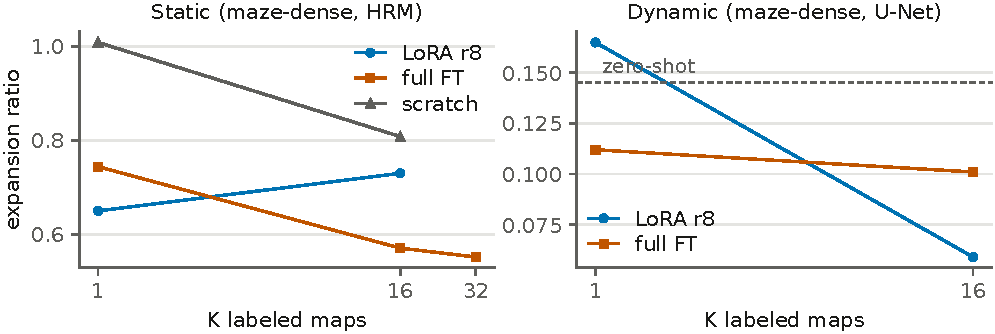
\includegraphics[width=0.98\textwidth]{figures/fig3_transfer.pdf}
\caption{Illustrative $K$-indexed adaptation curves on the static (left) and dynamic (right) dense-maze targets (moved from the main paper; the factorial figure there supersedes them as the primary adaptation visual). On this static target, LoRA leads at $K{=}1$ and full fine-tuning overtakes it by $K{=}16$; on the dynamic target the low-supervision failure is not observed in the $K$-indexed protocol. Curves connect the evaluated $K$ values for one backbone per panel; quoted inference is map-clustered.}
\label{fig:kcurves}
\end{figure*}

\begin{table*}[t]
\centering
\small
\setlength{\tabcolsep}{2.2pt}
\begin{tabular}{@{}lccc c@{}}
\toprule
Cell & $K$ & $\Delta$succ.\ [CI] & $\Delta$ratio [CI] & $n$ \\
\midrule
dense/HRM & 1 & $-.240$ $[-.360,-.133]$ & $+.112$ $[+.052,+.171]$ & 10 \\
dense/HRM & 16 & $+.027$ $[-.020,+.100]$ & $-.149$ $[-.179,-.117]$ & 10 \\
dense/ON-L. & 1 & $-.047$ $[-.147,+.073]$ & $-.162$ $[-.223,-.089]$ & 10 \\
dense/ON-L. & 16 & $+.000$ $[-.027,+.033]$ & $-.126$ $[-.171,-.083]$ & 10 \\
bug./HRM & 1 & $-.467$ $[-.587,-.340]$ & $+.225$ $[+.089,+.352]$ & 13 \\
bug./HRM & 16 & $-.020$ $[-.120,+.080]$ & $-.145$ $[-.239,-.043]$ & 16 \\
bug./ON-L. & 1 & $-.093$ $[-.207,+.007]$ & $+.229$ $[+.117,+.348]$ & 15 \\
bug./ON-L. & 16 & $+.100$ $[+.013,+.207]$ & $-.052$ $[-.154,+.033]$ & 15 \\
rl./HRM & 1 & $-.600$ $[-.773,-.407]$ & $+.290$ $[+.207,+.360]$ & 11 \\
rl./HRM & 16 & $+.073$ $[-.027,+.187]$ & $-.366$ $[-.489,-.235]$ & 11 \\
rl./ON-L. & 1 & $-.293$ $[-.433,-.160]$ & $+.013$ $[-.156,+.167]$ & 11 \\
rl./ON-L. & 16 & $-.053$ $[-.167,+.053]$ & $-.170$ $[-.326,-.010]$ & 11 \\
\bottomrule
\end{tabular}
\caption{Direct map-paired full-FT $-$ LoRA contrasts (dense = dense maze, bug.\ = bugtrap, rl.\ = large rooms; ON-L.\ = ON-LSTM). Adaptation seeds are averaged within maps; intervals are 10k map-clustered bootstraps over the 30 test maps per target; $\Delta$ratio is computed on the $n$ triple-matched maps solved by both methods and the anchor, as a difference of expansion ratios relative to the anchor (negative favors full fine-tuning). At $K{=}1$ the success contrast favors LoRA in all six cells (four intervals exclude zero); at $K{=}16$ the effort contrast favors full fine-tuning in all six cells (five intervals exclude zero) at near-parity success.}
\label{tab:directcontrast}
\end{table*}

Figure~\ref{fig:kcurves} shows the illustrative $K$-indexed curves and Table~\ref{tab:directcontrast} the direct map-paired method contrasts. Representative \stage{C9} HRM curves (ratio at success): maze-dense LoRA $0.650$ (1.00) at $K{=}1$ to $0.730$ (0.97) at $K{=}16$; maze-dense full FT $0.744$ (0.76) to $0.571$ (0.99) at $K{=}16$ and $0.552$ at $K{=}32$; scratch $1.008$ (0.37) to $0.808$ (0.80); rooms-large full FT $1.128$ (0.37) at $K{=}1$ to $0.500$ (0.92) at $K{=}8$. Bugtrap LoRA degrades from $\approx$0.696 (0.83) to $0.950$ (0.48) at $K{=}32$: LoRA is usually but not universally base-preserving. \stage{C9h} (matched compute): bounded-minus-unbounded LoRA median ratio delta $0.000\pm0.008$ across 27 cells (22/27 exactly zero; max $|\Delta|$ 0.028); rooms-large field U-Net full FT reaches $0.404$ at 0.97 success from $0.982$ zero-shot while conv-LoRA stays at $0.992$--$1.002$. \stage{C9b} (dynamics): maze-dense aware U-Net zero-shot $0.145$ (0.60), LoRA $K{=}16$ $0.059$ (0.97), full FT $K{=}1$ $0.112$ (0.70); aware-minus-blind success deltas at full-FT $K{=}16$ are $0.00$ or $-0.05$ in all nine cells. \stage{C10}: RBF-merge minus zero-shot expansion-ratio deltas by target/backbone: $-0.022$, $-0.012$, $-0.024$, $+0.082$, $+0.012$, $+0.116$; weight-space vs.\ prediction-space deltas lie within $[-0.012, +0.007]$; own-axis RBF mass 0.986--0.998.

\subsection{The matched-label factorial (C14)}

\begin{figure*}[t]
\centering
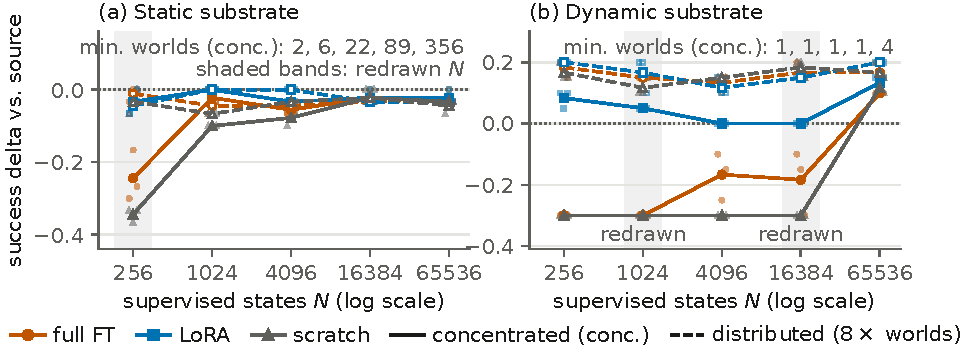
\includegraphics[width=0.98\textwidth]{figures/fig_c14_factorial.pdf}
\caption{The full matched-label factorial (both domains; the main paper shows the dynamic panel). Success delta versus the frozen zero-shot source at fixed supervised-state count $N$ on (a) the static and (b) the dynamic substrate. Solid: concentrated ($w_{\min}(N)$ worlds, annotated); dashed: distributed ($8\times$); small markers are the three adaptation seeds. Shaded bands mark the $N$ levels replicated with independent world draws (\stage{C14-R}).}
\label{fig:factorialfull}
\end{figure*}

A preregistered factorial (design and pre-execution amendment in the artifact package) tests whether the LoRA/full-fine-tuning contrast is governed by the number of supervised search states $N$, independent of domain and map count. Factors: $N \in \{256, 1024, 4096, 16384, 65536\}$ exact-count state samples $\times$ two coverage levels at fixed $N$ (concentrated: the minimal world count $w_{\min}(N)$; distributed: $8 \times w_{\min}(N)$ worlds) $\times$ two domains $\times$ \{unbounded rank-8 LoRA, full fine-tuning, scratch\} $\times$ 3 seeds. This yields 180 adaptations. Every cell runs an identical 2{,}560 optimizer steps and is evaluated on the frozen \stage{C9}/\stage{C9b} test cohorts at binding budgets. Sources are frozen: the \stage{C7} pooled scalar HRM base (static) and the \stage{C8} field U-Net blind twin (dynamic). The target is the maze-dense family in both domains. The measured $w_{\min}$ spans quantify the domains' supervision densities: reaching $N{=}65{,}536$ takes 356 static worlds but 4 dynamic worlds ($\sim$185 vs.\ $\sim$18{,}900 usable states per world).

\textbf{Preregistered primary hypothesis (H-C14): rejected as stated.} On matched-solved expansion ratios the hypothesized crossover point is degenerate: full fine-tuning is at or below LoRA at \emph{every} tested $N$ in all 12 (domain $\times$ coverage $\times$ seed) cells (dynamic ratio cells are descriptive at matched $n{=}1$; see Limitations), and the preregistered regression's full-FT $\times \log N$ interaction is null ($-0.0025$ $[-0.0087, +0.0028]$; Table~\ref{tab:c14reg}). State count improves ratios ($\log_2 N$ coefficient $-0.0140$ $[-0.0190, -0.0081]$) but identically for both methods. Ratios condition on jointly solved maps, so degraded-success cells can appear spuriously efficient; the factorial's conclusions therefore rest on success.

\textbf{The prespecified coverage readout identifies the supported success contrast.} LoRA's low-supervision advantage appears in \emph{success}, and it varies with distinct-world coverage at fixed $N$, not with state count (Table~\ref{tab:c14cells}; Figure~\ref{fig:factorialfull}). Concentrated low-world cells degrade full fine-tuning and scratch in both domains: success vs.\ the frozen zero-shot source is $-0.300$ $[-0.550,-0.050]$ in all three seeds at dynamic concentrated $N{=}256$ and $N{=}1{,}024$. At static concentrated $N{=}256$ the losses are $-0.167$ to $-0.300$ for full fine-tuning and $-0.333$ to $-0.367$ for scratch (every seed's CI excludes zero). The distributed cells at the same $N$ remove the deficit (dynamic $+0.150$ to $+0.200$; static $\approx 0.000$; paired dist$-$conc full-FT deltas $+0.45$ to $+0.48$ dynamic at these $N$, $+0.233$ static at $N{=}256$). At dynamic concentrated $N{=}16{,}384$ the full-fine-tuning deficit remains negative in every seed but excludes zero in only one of three. No LoRA cell has a harmful CI excluding zero (worst cell $-0.067$ $[-0.167, 0.000]$); the 60 per-cell readouts carry no multiplicity adjustment and no noninferiority margin, so this is a failure to observe degradation, not an equivalence claim. The dynamic concentrated arm recovers exactly where $w_{\min}$ forces multiple worlds ($N{=}65{,}536$, 4 worlds: $+0.100$ in all seeds); the recovery coincides with the forced rise in world count at fixed steps.

In the $K$-indexed adaptation protocols, map count and state count move together; the factorial separates them: held-out success varies with distinct-world coverage (or adapter-restricted capacity); raw state count does not explain it. Table~\ref{tab:c14cov} gives the direct distributed$-$concentrated contrast for every domain$\times N\times$method cell, with BH-adjusted sign-flip inference in the caption: for full fine-tuning and scratch, $q{<}0.05$ in all 10 cells with $w_{\min} \leq 2$ and in none of the 10 with $w_{\min} \geq 4$; LoRA's contrasts are small throughout, and its two marginally starred dynamic cells do not survive adjustment.

\begin{table*}[t]
\centering
\small
\setlength{\tabcolsep}{3.4pt}
\begin{tabular}{@{}lc ccc@{}}
\toprule
Domain & $N$ ($w_{\min}$) & Full FT & LoRA & Scratch \\
\midrule
static & 256 (2) & $+.233^{*}$ $[+.111,+.378]$ & $-.011$ $[-.067,+.044]$ & $+.311^{*}$ $[+.156,+.467]$ \\
static & 1024 (6) & $-.022$ $[-.056,+.000]$ & $.000$ $[.000,.000]$ & $+.033$ $[-.033,+.122]$ \\
static & 4096 (22) & $+.011$ $[-.033,+.067]$ & $+.033$ $[+.000,+.100]$ & $+.044$ $[+.000,+.122]$ \\
static & 16384 (89) & $-.011$ $[-.033,+.000]$ & $-.011$ $[-.033,+.000]$ & $.000$ $[.000,.000]$ \\
static & 65536 (356) & $+.011$ $[+.000,+.033]$ & $-.011$ $[-.033,+.000]$ & $-.011$ $[-.033,+.000]$ \\
dynamic & 256 (1) & $+.483^{*}$ $[+.283,+.700]$ & $+.117$ $[+.000,+.267]$ & $+.467^{*}$ $[+.250,+.683]$ \\
dynamic & 1024 (1) & $+.450^{*}$ $[+.250,+.650]$ & $+.117^{*}$ $[+.017,+.250]$ & $+.417^{*}$ $[+.217,+.633]$ \\
dynamic & 4096 (1) & $+.300^{*}$ $[+.133,+.483]$ & $+.117^{*}$ $[+.017,+.250]$ & $+.450^{*}$ $[+.250,+.650]$ \\
dynamic & 16384 (1) & $+.350^{*}$ $[+.183,+.533]$ & $+.150$ $[+.000,+.300]$ & $+.483^{*}$ $[+.283,+.700]$ \\
dynamic & 65536 (4) & $+.067$ $[+.000,+.183]$ & $+.067$ $[+.000,+.183]$ & $+.050$ $[+.000,+.133]$ \\
\bottomrule
\end{tabular}
\caption{Direct distributed$-$concentrated success contrasts, all 30 factorial cells: paired per-map differences with adaptation seeds averaged within maps and 10k map-bootstrap 95\% CIs (static $n{=}30$ maps, dynamic $n{=}20$). $^{*}$: marginal interval excludes zero. Adjusted inference (paired sign-flip tests, 20k flips, BH-corrected across the 30 cells): $q{<}0.05$ in exactly the 10 full-fine-tuning and scratch cells with $w_{\min} \leq 2$ (all $q \leq 0.032$), in none of the 10 with $w_{\min} \geq 4$, and in no LoRA cell (the two marginal LoRA cells rise to $q \geq 0.32$). The two-world threshold is a descriptive pattern identified post hoc, not a preregistered boundary.}
\label{tab:c14cov}
\end{table*}

\begin{table}[t]
\centering
\small
\setlength{\tabcolsep}{2.2pt}
\begin{tabular}{@{}llccc@{}}
\toprule
Dom./cov. & $N$ & Full FT & LoRA & Scratch \\
\midrule
static conc & 256 & $-.30\,$--$\,-.17^{*}$ & $-.07\,$--$\,.00$ & $-.37\,$--$\,-.33^{*}$ \\
static conc & 1024 & $-.03\,$--$\,.00$ & $.00$ & $-.10$ \\
static conc & 4096 & $-.07\,$--$\,-.03$ & $-.03$ & $-.10\,$--$\,-.07$ \\
static conc & 16384 & $-.03\,$--$\,.00$ & $-.03\,$--$\,.00$ & $-.03\,$--$\,.00$ \\
static conc & 65536 & $-.03$ & $-.03\,$--$\,.00$ & $-.03$ \\
static dist & 256 & $-.03\,$--$\,.00$ & $-.07\,$--$\,-.03$ & $-.07\,$--$\,.00$ \\
static dist & 1024 & $-.07\,$--$\,-.03$ & $.00$ & $-.07$ \\
static dist & 4096 & $-.07\,$--$\,-.03$ & $.00$ & $-.03$ \\
static dist & 16384 & $-.03$ & $-.03$ & $-.03\,$--$\,.00$ \\
static dist & 65536 & $-.03\,$--$\,.00$ & $-.03$ & $-.07\,$--$\,-.03$ \\
dynamic conc & 256 & $-.30^{*}$ & $+.05\,$--$\,+.10$ & $-.30^{*}$ \\
dynamic conc & 1024 & $-.30^{*}$ & $+.05$ & $-.30^{*}$ \\
dynamic conc & 4096 & $-.25\,$--$\,-.10$ & $.00$ & $-.30^{*}$ \\
dynamic conc & 16384 & $-.30\,$--$\,-.10^{\dagger}$ & $.00$ & $-.30^{*}$ \\
dynamic conc & 65536 & $+.10$ & $+.10\,$--$\,+.15$ & $+.10\,$--$\,+.15$ \\
dynamic dist & 256 & $+.15\,$--$\,+.20$ & $+.20$ & $+.15\,$--$\,+.20$ \\
dynamic dist & 1024 & $+.15$ & $+.10\,$--$\,+.20$ & $+.10\,$--$\,+.15$ \\
dynamic dist & 4096 & $+.10\,$--$\,+.15$ & $+.10\,$--$\,+.15$ & $+.15$ \\
dynamic dist & 16384 & $+.15\,$--$\,+.20$ & $+.15$ & $+.15\,$--$\,+.20$ \\
dynamic dist & 65536 & $+.15\,$--$\,+.20$ & $+.20$ & $+.15\,$--$\,+.20$ \\
\bottomrule
\end{tabular}
\caption{\stage{C14} per-cell success deltas versus the frozen source (range across the three adaptation seeds; a single value means all seeds agree). $^{*}$: the paired map CI excludes zero in the harmful direction in every seed. $^{\dagger}$: the CI excludes zero in one of three seeds. Per-seed CIs for all 180 cells ship in the artifact package.}
\label{tab:c14cells}
\end{table}

\begin{table}[t]
\centering
\small
\setlength{\tabcolsep}{3pt}
\begin{tabular}{@{}lc@{}}
\toprule
Term & Coefficient [95\% CI] \\
\midrule
intercept & $+0.7546$ $[+0.6969, +0.8198]$ \\
$\log_2 N$ & $-0.0140$ $[-0.0190, -0.0081]$ \\
full FT & $+0.0022$ $[-0.0691, +0.0842]$ \\
scratch & $-0.0213$ $[-0.0402, -0.0050]$ \\
dynamic & $-0.4387$ $[-0.4901, +0.0000]$ \\
distributed & $+0.0012$ $[-0.0197, +0.0205]$ \\
full FT $\times \log_2 N$ & $-0.0025$ $[-0.0087, +0.0028]$ \\
full FT $\times$ dynamic & $-0.0409$ $[-0.0585, +0.0000]$ \\
\bottomrule
\end{tabular}
\caption{\stage{C14} preregistered map-level regression of the matched expansion ratio on $\log_2 N$, method, domain, and coverage (map-clustered bootstrap CIs). H-C14 required the full-FT $\times \log_2 N$ interaction to be significantly negative; it is null.}
\label{tab:c14reg}
\end{table}

\textbf{Protocol detail.} Measured minimal world counts $w_{\min}(N)$ for $N{=}256/1{,}024/4{,}096/16{,}384/65{,}536$: static concentrated 2/6/22/89/356 worlds (distributed $8\times$: 16/48/176/712/2{,}848); dynamic concentrated 1/1/1/1/4 (distributed 8/8/8/8/32). In the dynamic domain, rank-8 LoRA wraps every Conv2d weight of the field U-Net with a shape-agnostic adapter parametrization (zero-initialized $B$, so the adapter is the identity at start; 20 wrapped convolutions; 192{,}080 trainable $A$/$B$ parameters, 5.2\% of the 3{,}702{,}370-parameter frozen base); the static domain uses the scalar HRM's rank-8 linear adapters. Every adaptation runs exactly 2{,}560 optimizer steps (the epoch-equivalent of the largest $N$ under the canonical recipe), so compute cannot proxy for labels; smaller-$N$ cells cycle their fixed sample. The three adaptation seeds vary initialization and batch order only; the sampled state indices are shared across methods and seeds within a cell. \emph{Degradation} denotes a cell whose adapted success falls below the trained source model's zero-shot success with the paired map CI excluding zero in the harmful direction; we reserve \emph{collapse} for the constant-prediction optimization failures of Sections~E and~I. Inference unit: evaluation maps, seeds averaged within maps.

\textbf{Limitations.} Euclid solves 1/20 dense dynamic test maps at the binding budget, so dynamic matched-ratio cells have $n{=}1$ and carry no map-level uncertainty; dynamic inference rests on the 20-map paired success deltas. One target family per domain; three adaptation seeds; the coverage factor counts distinct procedural worlds and does not measure geometric diversity; matching covers retained labels and optimizer steps, not the cost of generating and labeling additional worlds. Adaptations ran on cloud L4 hardware from locally collected, hash-recorded datasets.

\textbf{Targeted independent world-draw replications (C14-R; frozen design 2026-07-25).} Each original cell used one deterministically sampled world set; C14-R re-draws the world streams independently (draw offsets entering only the pool seeds; test cohorts, budgets, and sampling rules unchanged). The redraws target the decisive cells: dynamic $N \in \{1024, 16384\}$ and static $N{=}256$, both coverage levels, all three methods, one optimization seed, 18 arms per draw on the same frozen test cohorts. Results across both draws are deltas versus the frozen source with map-level CIs, reported as-is against the preregistered readouts; the original factorial's world sets are draw 1, the redraws draws 2 and 3. \emph{All 18 targeted redraw contrasts are positive}: CIs exclude zero for scratch in all six (up to $+0.500$) and for full fine-tuning in five of six. The full-fine-tuning contrasts are draw 2 dynamic $+0.350$ $[+0.150,+0.550]$ and $+0.200$ $[+0.050,+0.400]$, and draw 3 dynamic $+0.400$ $[+0.200,+0.600]$ and $+0.300$ $[+0.100,+0.500]$ with static $+0.133$ $[+0.033,+0.267]$; the exception is draw 2's static contrast, $+0.067$ $[+0.000,+0.167]$, whose lower bound touches zero. Every targeted distributed arm improves on its concentrated counterpart (R2 passes twice).

\emph{Concentrated harm is directionally consistent but power-limited for full fine-tuning}: scratch's dynamic concentrated harm excludes zero in both draws ($-0.300$ $[-0.550,-0.050]$ each). Full fine-tuning's harm reproduces in sign and magnitude ($-0.200$ and $-0.250$ at $N{=}1024$) but its CIs graze zero at $n{=}20$ maps and one optimization seed, so strict R1 fails in both draws. \emph{The harm's magnitude depends on the drawn worlds}: draw 3's static concentrated cells are harmful with CIs excluding zero for all three methods (full FT $-0.233$; scratch $-0.500$; LoRA $-0.133$ $[-0.267,-0.033]$, failing R4; the first LoRA degradation in the factorial family whose CI excludes zero (\stage{C9}'s bugtrap $K{=}32$ cell is the program's other; Table~\ref{tab:wcr-c9}), still the least-degraded method in its cell). Draw 2's static concentrated worlds happen to be benign (full FT $-0.067$, n.s., failing R3; LoRA never degrades in draw 2, passing R4).

Synthesis: positive coverage contrasts recur under independent world draws; the concentrated-harm magnitude varies with which worlds are drawn; and LoRA is generally the least-degraded method in the tested low-coverage cells, though not absolutely: across the original factorial and both replicates, exactly one LoRA cell (draw 3, static concentrated) degrades with a CI excluding zero. Raw rows for both draws ship in the artifact package.

\section{E. \stage{C11} Gates, Collapse Forensics, and Scale}

Figure~\ref{fig:c11} shows the oracle-headroom and learned-halting views summarized in the main paper, and Table~\ref{tab:c11gates} records the preregistered gate verdicts.

\begin{figure*}[t]
\centering
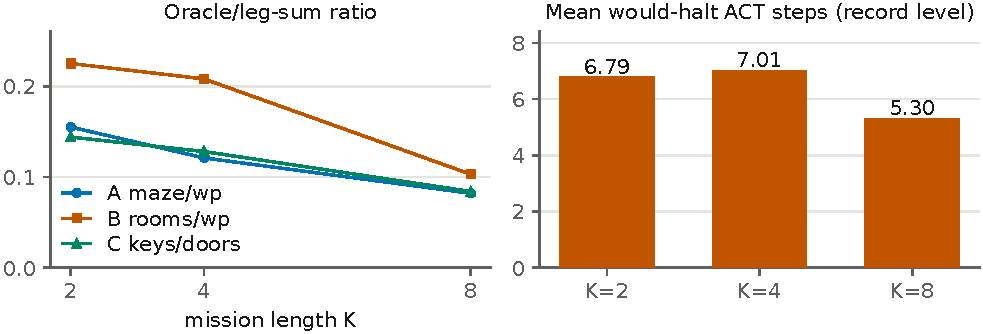
\includegraphics[width=0.98\textwidth]{figures/fig4_c11.pdf}
\caption{Compositional-mission hierarchy test (\stage{C11}); $K$ here is mission length. Left: the exact oracle's ratio over a leg-sum baseline falls as missions deepen (headroom exists). Right: learned HRM halting uses \emph{fewer} steps at $K{=}8$; bar labels are record-level means (map-level 6.78/7.01/5.30); both analysis grains: map-level $\rho=-0.578$, $p=5\times10^{-5}$, $n{=}225$ maps; record-level $\rho=-0.407$, $n{=}675$.}
\label{fig:c11}
\end{figure*}

\begin{table}[t]
\centering
\footnotesize
\begin{tabular}{@{}lp{5.2cm}@{}}
\toprule
Gate & Verdict \\
\midrule
K=0 continuity & FAIL, diagnosed as false premise: \stage{C7} had no MLP arm and did not give every architecture the \stage{C11} input; real shallow separation plus collapsed recurrent cells violate the all-tie assumption. Measurement layer verified. \\
G1 dose--response & Negative: no structured arm beats MLP at $\geq$2 mission depths with non-decreasing gap. \\
G2a forced compute & Negative: HRM-v2 $k{=}1/2/4/8$ expansion and MAE curves flat in every $K{=}8$ config. \\
G2b learned halting & Negative, inverted: map-level Spearman $\rho{=}-0.578$, stratified permutation $p{=}5{\times}10^{-5}$, $n{=}225$ maps (record-level $\rho{=}-0.407$, $n{=}675$, the original gate value); mean would-halt steps 6.79/7.01/5.30 at $K{=}2/4/8$ (record level; map level 6.78/7.01/5.30). \\
G3 closure & Neither preregistered branch: global-input arms separate at shallow $K$ (U-Net/GNN vs.\ MLP ratios $\approx$0.67--0.87 at record level, map-clustered values in Section~J; state MAE 0.151/0.171 vs.\ 0.251 at A/$K{=}0$), but no arm converts depth into growing advantage. \\
\bottomrule
\end{tabular}
\caption{\stage{C11} preregistered gate verdicts. The criteria (the $K{=}0$ continuity check, depth dose--response G1, compute conversion G2a/G2b, closure G3) were frozen before evaluation; each row summarizes the registered outcome. Map-clustered companion values are in Section~J.}
\label{tab:c11gates}
\end{table}

\textbf{Collapse forensics.} Five of 33 recurrent/ACT arm-cells show constant-prediction or partial seed collapse (HRM-trace A8/C8, ON-LSTM B0, HRM-v2 B0, two ON-LSTM A8 seeds), with a reproducible loss signature at the normalization cap. The largest recurrent deficits (HRM-trace ratios 1.526 at A8, 1.600 at C8) are collapse measurements, not expressiveness estimates. Removing $K{=}0$ padding \emph{worsens} recurrent predictions: models used pad steps as extra recurrent compute.

\textbf{Scaled addendum.} A 12-run \texttt{unet\_film\_big} vs.\ \texttt{hrm\_trace\_big} comparison (complete; 2{,}700 eval rows) preserves the ordering: completion 0.804 vs.\ 0.736 at $K{=}2$ and 0.413 vs.\ 0.307 at $K{=}8$; mean state MAE 0.395 vs.\ 0.447 ($K{=}2$) and 0.906 vs.\ 1.855 ($K{=}8$). At $K{=}8$ the scaled HRM exactly matches the leg-sum baseline's completion and mean expansions (0.307; 701.34)---persistent collapse, not recovered hierarchy.

\section{F. \stage{C12} Detail}

\stage{C12-A} (memory headroom, then learned pilot): constructed decision-relevant aliasing at 71.3\% of paired decisions; privileged mode/history diagnostic $+0.467$ completion and a 65.1\% collision-adjusted regret reduction (map-bootstrap 95\% CI 63.0--66.9\%); oracle completion 0.975. The one-seed matched temporal-hierarchy pilot fails G1 (forecast), G2 (planning), and G3 (persistent carry); overall a strong negative result. \stage{C12-B} (tied refiner): cycle-1$\to$8 normalized burden improves monotonically in every cell (A/$K2$ 0.859$\to$0.815; A/$K8$ 0.624$\to$0.576; C/$K2$ 0.867$\to$0.777; C/$K8$ 0.576$\to$0.517; all cycle-1/8 map-bootstrap intervals separate), but the $K8{-}K2$ gain is $+0.0038$ (CI $[-0.0199, 0.0281]$) on A and $-0.0305$ ($[-0.0726, 0.0096]$) on C: no dose--response. Tied beats shallow and untied on C/$K8$ (deltas 0.0177/0.0076, BH $q{=}6.7{\times}10^{-5}$) but loses to untied on A/$K8$ ($q{=}0.0168$). Bellman residual \emph{worsens} over cycles in every cell while burden improves; solved cycle-8 paths average 1.4--2.2\% above oracle cost. $K{=}16$ was dropped before training by a pre-specified construction check (only 2/300 and 1/300 valid missions).

\section{G. C13: Mechanism Ladder and Frozen Confirmation}

\textbf{Claim supported.} With one inference-time local Bellman backup and a frozen scale calibration, a provider restricted to bounded local observations (radius-0.20 subgraph on a known roadmap; behavior-derived labels; no shortest-path supervision) beats every fixed complete-map \stage{C7} provider in pooled expansions, at matched empirical path quality, on a frozen disjoint cohort.

\textbf{Ladder.} Each step changes one factor (Table~\ref{tab:c13ladder}); deltas are paired expansions versus the matched comparator (steps C--G versus matched focal search at $w{=}1.10$ on six development maps, steps C--D using exact oracle values; steps I--M versus the complete-map field HRM, live on all six suites).

\begin{table}[t]
\centering
\small
\setlength{\tabcolsep}{1.5pt}
\begin{tabular}{@{}llr@{}}
\toprule
Step & Factor changed & $\Delta$ exp.\ [CI] / (wins) \\
\midrule
C & fresh certifier (oracle rank) & $+11.50$ (0/6) \\
D & shared-queue certifier (oracle) & $-6.83$ (6/6) \\
E & exact rollout rank & $+1.33$ (2/6) \\
F & monotone recalibration & $+1.33$ (2/6) \\
G & analytic local escape & $+6.83$ (0/6) \\
I & one-family model, live 6 suites & $+15.36$ $[+12.02,+18.64]$ \\
J & suite-balanced, static insert & $+16.17$ $[+9.67,+22.67]$ \\
K & + one local Bellman backup & $-1.21$ $[-8.04,+5.46]$ \\
L & + scale $\alpha{=}1.5$ (48 maps) & $-13.04$ $[-18.67,-7.65]$ \\
M & frozen 144-map confirmation & $-12.96$ $[-16.30,-9.74]$ \\
\bottomrule
\end{tabular}
\caption{The \stage{C13} falsification ladder. Target repairs (E, F), analytic constructions (G), and distribution repairs (I, J) fail; the integration repair (K) plus scale calibration (L) flip the sign, and the frozen confirmation (M) reproduces it. Steps C--D are oracle-value diagnostics that bound what certification alone achieves, not live-model arms. Steps \stage{A} (state-semantics and density audit) and \stage{B} (fresh-start rollout labeling) are construction stages with no search arm, and \stage{H} is the maze-only feasibility gate for local Bellman learning that motivated \stage{I}--\stage{M}; none yields a paired delta, so they carry no rows. \stage{N}--\stage{P} are separate post-confirmation studies, not ladder steps.}
\label{tab:c13ladder}
\end{table}

\textbf{Frozen confirmation, per suite.} 144 maps (24 per family; seeds disjoint from every prior cohort; feature caches hash-verified against live regeneration; model, radius 0.20, $\alpha{=}1.50$, integration, and analysis frozen before generation). Table~\ref{tab:c13msuite} gives the per-suite outcomes.

\begin{table*}[t]
\centering
\small
\setlength{\tabcolsep}{2.5pt}
\begin{tabular}{@{}lrrrlr@{}}
\toprule
Suite & Local & Field HRM & $\Delta$ & 95\% CI & W/T/L \\
\midrule
Maze & 47.63 & 84.38 & $-36.75$ & $[-45.58,-27.83]$ & 24/0/0 \\
Dense maze & 95.38 & 104.50 & $-9.13$ & $[-15.21,-3.13]$ & 18/1/5 \\
Rooms & 98.04 & 106.17 & $-8.13$ & $[-14.33,-1.71]$ & 16/0/8 \\
Spiral & 120.25 & 121.33 & $-1.08$ & $[-5.88,+4.21]$ & 14/1/9 \\
Bugtrap & 14.96 & 24.29 & $-9.33$ & $[-17.79,-2.92]$ & 18/1/5 \\
Large rooms & 33.58 & 46.92 & $-13.33$ & $[-18.92,-7.50]$ & 19/0/5 \\
\midrule
Pooled & 68.31 & 81.26 & $-12.96$ & $[-16.30,-9.74]$ & 109/3/32 \\
\bottomrule
\end{tabular}
\caption{\stage{C13-M} per-suite paired expansion deltas versus the complete-map field-HRM comparator. Every suite mean is negative; the spiral interval crosses zero, and the preregistered criterion pools all suites with a suite-breadth condition (at least four negative suite means), which passes. The local provider also beats every other fixed \stage{C7} learned provider in pooled expansions on this cohort.}
\label{tab:c13msuite}
\end{table*}

\textbf{Scale calibration.} On the disjoint 48-map calibration block, $\alpha\in\{1.00,1.25,1.50,2.00\}$ gives deltas $-3.79$ $[-9.40,+1.73]$, $-9.77$ $[-15.38,-4.42]$, $-13.04$ $[-18.67,-7.65]$, and $-16.94$ $[-22.56,-11.54]$, with 4/4/6/6 negative suite means and mean/max cost ratios rising from 1.022/1.241 to 1.052/1.366. $\alpha{=}1.50$ was frozen as the largest scale whose calibration-block cost stayed within the comparator-relative margins ($\alpha{=}2.00$'s mean ratio exceeds the field HRM's 1.042 by $+0.010$, beyond the $+0.005$ margin; both scales reach 6/6 suite breadth). Every arm formally fails the preregistered absolute 1.10 maximum-cost ceiling. \emph{Chronology, stated explicitly:} the absolute ceiling was part of the original calibration design, and its failure was observed on the calibration block, during development, before any confirmation data existed. The comparator-relative criterion (mean path-cost ratio within $+0.005$ and maximum within $+0.02$ of the complete-map field HRM) and the $\alpha{=}1.50$ selection were then written into the frozen confirmation design \emph{before} the 144-map cohort was generated. No criterion changed afterward. Under that criterion the confirmation passes with margin (1.0235/1.1624 vs.\ 1.0311/1.3346); had the original absolute ceiling been retained, the direct arm would fail it on maximum cost, which we report rather than suppress.

\textbf{Operating points and timing.} The direct $\alpha{=}1.50$ arm is the matched-quality expansion result and carries no formal bound. The separate certified operating point runs the learned rank inside a $w{=}1.10$ focal band with a shared-queue consistent-bound incumbent proof and passes all 144 bound and certificate checks. Per-map wall time decomposes as feature construction 5.138\,s (prototype Python builder), model inference 0.0008\,s, local backup 0.0097\,s, and search 0.0002\,s, versus 0.371\,s complete-map field-HRM inference: the result is search effort and path quality, not latency.

\textbf{Architecture substitutions (\stage{C13-N}/\stage{O}) and the persistent-state pilot (\stage{C13-P})} are summarized in the main paper; their raw artifacts (development grids, recorded outcomes, integrity manifests) ship in the artifact package.

\section{H. Discrete Program Detail}

The discrete program is larger than the canonical subset reported here: fifteen experiment families, including forecaster lineages, diffusion baselines, an empty-model baseline-rerun control, and a budget-invariance analysis showing that raising budgets adds work without rescuing success on the hard families. The paragraphs below report the completed canonical results; the full inventory ships with the released artifacts.

\textbf{Forecasting.} Matched 100-episode protocol: HRM-3M/10M 71/100 vs.\ LSTM 67--69/100 (no uncertainty reported; two-episode matched gap). Structured Preset~M+ (four 100-episode suites): ON-LSTM-10M 0.3875 mean success vs.\ HRM-10M 0.2650 and HRM-3M 0.200; the ON-LSTM family also leads rollout MSE, the 3M variant lowest (0.1257/1.1269 one-/five-step vs.\ 0.3973/2.6438 for HRM-3M).

\textbf{Additive transfer (clean v3, 22 suites $\times$ 3 budgets).} Manhattan 0.590 success / 126{,}707 mean expansions; HRM full-FT 0.585 / 128{,}013; ON-LSTM full-FT 0.564 / 127{,}228; HRM LoRA 0.554 / 140{,}852; ON-LSTM LoRA 0.514 / 145{,}282. Every learned arm $\leq$ matched baseline.

\textbf{Pooled multitask.} HRM pooled base 0.612 success ($+2.11$pp) / 122{,}184 expansions vs.\ Manhattan 0.591 / 126{,}630, the strongest completed discrete additive positive; only 1 of several specialists beats its matched four-suite baseline ($+2.0$pp; others $-0.42$ to $-20.25$pp).

\textbf{Focal ranking (local pilot, 3--8 seeds).} Magnitude is scale-flat despite near-perfect ordering (correlation 0.987--0.994; predicted/true mean 0.73/0.42/0.27/0.19 at 64/128/192/256). At $w{=}1.0$: HRM A128-static ratio 0.85 with success 0.62$\to$0.75; A192 0.94 (0.75$\to$0.75); A128-dynamic 0.93 (0.62$\to$0.62); ON-LSTM A128/A192 0.85 (0.75$\to$0.75). At $w{=}1.05$, A128-dynamic improves further but A192 success regresses 0.75$\to$0.62; $w{=}1.0$ is the evidence-safe operating point. Experts exactly match pooled bases in tested cells.

\section{I. Validity Forensics}

\textbf{The frozen-halt artifact.} An early discrete adaptive-computation run reported ``74.60\% halt accuracy'' that equals $100$ minus the run's exact-solve accuracy: the halt logit was frozen (the training loop omitted the halt loss), so the metric measured a constant never-halt classifier. The loss path was repaired and verified live; we note the $100{-}x$ pattern as a red flag for adaptive-computation metrics, and no main-paper claim uses this run.

\textbf{The cap-collapse signature.} \stage{C5}'s scalar HRM collapse sits at a loss value pinned by the residual cap (2.612 in that setup, with constant predictions at the cap). The same class of signature reappears in \stage{C11}: collapsed cells share an \emph{identical} final loss (1.1397, exactly the constant-cap loss under that normalization), enabling automatic collapse detection instead of misreading collapsed cells as capacity evidence.

\textbf{Pad steps as compute.} In \stage{C11}, removing $K{=}0$ padding tokens \emph{degraded} recurrent predictions: models had co-opted padding as additional recurrent iterations. Sequence-model comparisons that alter padding alter compute.

\section{J. Statistics and Map-Clustered Reanalysis}

\textbf{Primary-test policy.} Exact McNemar with BH correction is the primary success test within each experiment's set of suites. Paired bootstrap intervals are descriptive companions, and where a marginal interval excludes zero but the corrected test does not (crossing, under the weighted-A\textsuperscript{*} control), the corrected test governs. Matched-ratio and path-quality intervals are marginal and uncorrected unless stated otherwise. The 30 direct \stage{C14} coverage contrasts also carry paired sign-flip randomization tests (20k flips, seeds averaged within maps) with BH correction across the 30 cells (Table~\ref{tab:c14cov} caption). Chronology: the distributed$-$concentrated success contrast is the prespecified secondary endpoint; the sign-flip/BH test family was added after completion, during review response, as a multiplicity-controlled reanalysis; it does not inherit preregistered status. Multiplicity families are declared per experiment: the six static or dynamic suites of each zero-shot or control comparison, the six target/backbone cells per endpoint and $K$ for the direct method contrasts, and the six suites of the \stage{C13} confirmation.

Expansion effort is compared only on matched solved maps via median ratios with bootstrap percentile CIs (10k--20k resamples); from \stage{C12} onward, bootstraps are map-clustered by design. \stage{C9}--\stage{C11} originally pooled repeated evaluations of fixed test maps across adaptation/model seeds; the reanalysis below covers every quantity the main paper quotes from those stages; the fixed-provider dynamic reanalysis of Table~\ref{tab:c8fixed} uses the same map-level grain. Matched-solved ratios condition on joint success and can favor arms that solve only easier maps; we therefore always report success and ratios separately and never combine them into a single score. Negative results are failures to observe an effect under the tested protocol, not equivalence claims; no equivalence tests were run.

\subsection{Map-clustered reanalysis}

Units are test maps, and adaptation/model seeds are averaged within maps before inference. Success deltas use 10{,}000-resample map bootstraps; expansion ratios are medians of per-map ratios over matched maps at the binding budget in additive mode. The \stage{C11} halting test aggregates model seeds within maps and permutes mission length within config (maps are independent across $K$ cells; 20{,}000 stratified permutations). Estimator conventions differ slightly from the published record-level curves, so point values differ modestly; the question is whether the conclusions agree. A methodological caution surfaced during this work: a first pass that accidentally pooled additive and focal evaluation modes attenuated the apparent \stage{C9} transfer effects by roughly half. Mode and aggregation mixing alone can materially change an apparent effect of the size under study.

\textbf{\stage{C11} halting.} Record level reproduces the originally recorded value ($\rho{=}-0.4066$, $n{=}675$); map level strengthens it ($\rho{=}-0.5778$, $n{=}225$, stratified permutation $p{=}5{\times}10^{-5}$). Map-level means 6.78/7.01/5.30 at $K{=}2/4/8$.

\textbf{\stage{C11} vs-MLP ratios.} Map-clustered ratio-of-means CIs exclude parity at $K\in\{0,2\}$ in config A for both U-Net (0.734/0.846) and GNN (0.822/0.923), and in config B at $K{=}0$ (U-Net 0.904, GNN 0.818) plus B/$K{=}2$ for the GNN (0.805); config C never separates; every $K\in\{4,8\}$ cell includes parity.

\begin{table}[t]
\centering
\small
\setlength{\tabcolsep}{1.5pt}
\begin{tabular}{@{}lll@{}}
\toprule
Cell (HRM) & $\Delta$succ.\ [CI] & map ratio [CI] \\
\midrule
dense LoRA $K{=}1$ & $+0.47$ $[+0.30,+0.63]$ & 0.69 $[0.59,0.77]$ \\
dense LoRA $K{=}16$ & $+0.43$ $[+0.27,+0.60]$ & 0.79 $[0.69,0.89]$ \\
dense full $K{=}1$ & $+0.23$ $[+0.08,+0.38]$ & 0.79 $[0.75,0.84]$ \\
dense full $K{=}16$ & $+0.46$ $[+0.29,+0.63]$ & \textbf{0.61} $[0.55,0.67]$ \\
dense scratch $K{=}1$ & $-0.17$ $[-0.30,-0.05]$ & 1.04 $[1.03,1.04]$ \\
rl.\ full $K{=}1$ & $-0.17$ $[-0.34,+0.01]$ & 1.29 $[1.17,1.50]$ \\
rl.\ full $K{=}8$ & $+0.39$ $[+0.23,+0.55]$ & 0.59 $[0.50,0.71]$ \\
bug.\ LoRA $K{=}32$ & $-0.32$ $[-0.51,-0.13]$ & 1.15 $[1.01,1.52]$ \\
\bottomrule
\end{tabular}
\caption{Map-clustered \stage{C9} key cells (binding budgets, additive mode; dense = maze-dense, rl.\ = rooms-large, bug.\ = bugtrap; rounded to two decimals here, three-decimal values in the text and artifact). The $K{=}16$ full-FT/LoRA CIs are disjoint (the crossover; bold marks its ratio), the rooms-large $K{=}1$ degradation excludes parity, and the bugtrap LoRA degradation excludes zero in both metrics.}
\label{tab:wcr-c9}
\end{table}

\textbf{\stage{C9h} bound-vs-capacity.} 27 cells: median bounded-minus-unbounded map-level ratio delta $+0.0000$; 15/27 exactly zero; sd 0.0077; max $|\Delta|$ 0.0370---the capacity attribution stands.

\textbf{\stage{C9b} aware$-$blind (full FT, $K{=}16$).} Eight of nine point deltas are zero or negative; the single positive ($+0.017$ $[0.000,+0.050]$) does not exclude zero; no cell's interval favors the aware twin.

\textbf{\stage{C10} composition.} Map-paired expansion-ratio deltas vs.\ zero-shot (positive = more expansions): four cells $\approx$0 with CIs crossing zero; the two ON-LSTM rooms cells are \emph{worse} with CIs excluding zero ($+0.089$ $[+0.061,+0.121]$ and $+0.098$ $[+0.076,+0.123]$), matching the published point deltas and upgrading the null to ``never better, sometimes worse.''

No preregistered conclusion flips under any of these recomputations.

\section{K. Reproducibility and Artifact Inventory}

From \stage{C7} onward every stage freezes a written design (gates, budgets, analysis grain) before execution, and artifacts (checkpoints, feature caches, cohort manifests, raw rows, verdicts, reports) are hash-bound in integrity manifests. Confirmation cohorts are generated only after freezing model, integration, and evaluation code; failed development gates block confirmation rather than triggering retuning. Duplicate-evaluation determinism is enforced where preregistered (byte-identical traces; identical decision rows). The final-stage pilot on persistent planning-time state (\stage{C13-P}) ran under a fully test-verified harness (158 focused-plus-neighboring tests; hardware preflight). Its first staged execution ended at a preregistered execution-integrity hard stop: the harness's independent reanalysis disagreed with the primary comparison computation, voiding that execution's recorded metrics. After repair of the named defect only, a fresh-fingerprint rerun passed every integrity primitive, including independent reconstruction of the comparison evidence from promoted raw artifacts. It returned the valid negative reported in the main paper: persistent carry loses to the same-checkpoint reset twin at ranking frontier nodes on recorded search events (map-macro mean reciprocal rank of the labeled node; MRR delta $-0.029$, 95\% CI $[-0.060,-0.003]$). No follow-on self-training or confirmation stage was run. We note the initial stop as the integrity machinery functioning as designed.

The anonymized artifact archive submitted with this paper contains:
\begin{itemize}
    \item \emph{Analysis scripts} that regenerate the quoted map-level statistics from raw rows: the fixed-provider dynamic reanalysis, the map-clustered reanalysis, the weighted-A\textsuperscript{*} analysis (exact McNemar, ratio CIs, matched path quality), the budget-curve derivation, the reachable-label recount, the factorial and coverage analyses, the MovingAI external-benchmark, probe, and few-shot adaptation analyses, and all figure generators.
    \item \emph{Raw paired evaluation rows, zero-shot and controls}: \stage{C7}/\stage{C8} evaluation tables with the fresh-cohort and both retrained-pipeline replication rows; weighted-A\textsuperscript{*} development and confirmation rows with the tuned-weight manifest, plus the extended-grid rows and selection report; SIPP rows with per-instance correctness checks and timings (corrected-cohort and voided sibling-cohort sets, per the erratum); MovingAI external rows with the map manifest, the probe and few-shot adaptation rows, and the wall-time sample.
    \item \emph{Raw paired evaluation rows, adaptation}: \stage{C9}/\stage{C9h}/\stage{C9b}/\stage{C10} evaluation tables; \stage{C14} per-cell outputs with sampled-index manifests, the measured $w_{\min}$ stream, and the 30-cell coverage contrasts with their BH-adjusted sign-flip companion; and the \stage{C14-R} targeted redraws.
    \item \emph{Raw paired evaluation rows, remaining stages}: \stage{C11} evaluation and halting tables, \stage{C12} refiner and memory-pilot test tables, \stage{C13} development and confirmation rows, and the discrete-program summary tables.
    \item \emph{Manifests and configuration:} map/cohort manifests, seed lists, frozen configurations, the binding-budget calibration file, the serialized-world hash manifest for the 300-instance confirmation cohort, and the integrity manifests for the frozen confirmations.
    \item \emph{Generators and constructors:} the procedural world generator, model constructors, and the MovingAI conversion rule with its map manifest.
    \item \emph{Preregistration documents} from \stage{C7} onward, including the \stage{C14} design with its pre-execution amendment and post-completion supersession record, the 2026-07-25 SIPP, MovingAI, and \stage{C14-R} designs, the 2026-07-26 extended-grid design with its disclosed chronology, and the 2026-07-27 probe/few-shot design.
    \item \emph{Checkpoints:} the two frozen sources the headline claims rest on (the fixed dynamic provider and the frozen static adaptation source); all other checkpoints are regenerable from the recorded commands and seeds.
    \item \emph{Scale and external-map studies (Section~L):} \stage{C8-S} evaluation, probe, and sensitivity rows with randomized timing repeats, the 24-cell timing-multiplicity and slope-contrast analyses, and per-size calibration and tuning reports; \stage{C8-X} zero-shot rows and all 192 adaptation-cell rows with balanced-draw manifests, exact retained-label masks with the SHA-256 dataset/checkpoint manifest, conversion-fidelity metrics, pool/held-out map manifests, and the resharded evaluation parts with merge outputs; both frozen designs with dated amendments.
    \item \emph{A top-level README} with reproduction recipes and expected outputs; it states explicitly that analysis-script path constants must be pointed at the package's raw directories when running standalone.
\end{itemize}

\section{L. Scale and External-Map Studies}

Both studies run under frozen preregistered designs with dated amendments (every deviation disclosed) and freeze the paper's exact dynamic artifact (the blind U-Net checkpoint, SHA-verified at load; additive integration).

\begin{table}[t]
\centering
\small
\setlength{\tabcolsep}{2.6pt}
\begin{tabular}{@{}lccc@{}}
\toprule
$N$ & R1 (frozen) & Ratio range & Crossover \\
\midrule
192 & PASS 5/6 & .062--.249 & --- \\
512 & PASS 5/6 & .075--.183 & spiral (GPU) \\
1024 & FAIL 4/6 & .072--.216 & spiral (GPU+CPU) \\
2048 & FAIL 3/6 & .101--.285 & --- \\
\bottomrule
\end{tabular}
\caption{\stage{C8-S} summary. R1 = preregistered success-breadth criterion; failures arise only from floor/ceiling operating points. Ratio range = defined matched learned-to-anchor expansion-ratio medians. Crossover = suites meeting the frozen wall-time criterion at that size (BH $q{=}0.0002$ over the 24-cell scan).}
\label{tab:c8s-summary}
\end{table}

\textbf{Scale study (C8-S).} One shared fresh cohort per suite (10 dev +
30 eval worlds), each world accepted only if its roadmap builds and
connects at all of $N \in \{192, 512, 1024, 2048\}$ (per-size rebuilds,
not nested prefixes; the paired unit is the world). Budgets scale with
$N$; the anchor-only calibration and weighted-A\textsuperscript{*} tuning
are re-run per size and suite on dev worlds. Arms: anchor, tuned
WA\textsuperscript{*}, learned (CPU and GPU, identical code path), and
SIPP; three timing repeats, randomized arm order, warmup and roadmap construction excluded. Success persistence passes its
preregistered $\geq$5/6-suite bar at 192 and 512 and fails it at 1024 and
2048 solely through floor and ceiling cells (Table~\ref{tab:c8s-summary}): the frozen closest-target
rule targets anchor operating points (0.06/0.16) below the 10-world dev
resolution, a calibration failure mode at scale. Every non-degenerate
learned-versus-anchor success cell at every size is BH-significant
($q<0.01$; maze $+0.93$ and crossing $+0.80$ at $N{=}2048$). A post-hoc sensitivity pass (smallest ladder budget with dev anchor success in $[0.30, 0.70]$) renders four of the seven degenerate cells discriminative in the learned method's
favor with zero reverse-discordant maps (dense $+0.57/+0.70/+0.50$ at
192/512/1024, tying re-tuned WA\textsuperscript{*}; rooms-large@1024
$+0.53$, above the original-binding WA\textsuperscript{*} by $+0.23$);
three 2048 cells remain uninformative (the anchor's budget curve jumps
the band). Matched expansion ratios stay 0.062--0.285 with CIs below one
at every size. The preregistered wall-time crossover criterion (paired
learned$-$WA\textsuperscript{*} time CI below zero, success noninferior
within 0.05, path within $+0.02$) is met on spiral at $N{=}512$ (GPU;
$-1.19$\,s $[-1.82,-0.57]$, success $+0.17$) and persists at 1024
($-5.64$\,s); BH across all 24 suite$\times$size contrasts gives
$q{=}0.0002$ for both cells (the crossover rule was preregistered; the BH companion is a post-completion multiplicity check). No other suite crosses by 2048. Estimated
log-log wall-time slopes are 0.62--0.91 (learned GPU) versus 1.27--1.66
(WA\textsuperscript{*}); paired world-bootstrap slope contrasts ($+0.36$ to $+1.02$) exclude zero on every non-degenerate suite. SIPP reaches the feasibility ceiling under the implemented model
(0.97--1.00) with wall time exceeding the learned GPU arm's at 2048 in
every suite under their respective protocols (own units, never merged;
not a success- or resource-matched comparison). The residual probe's rank correlation stays stable across the tested sizes while its bias grows more negative. CPU and GPU
agree on success in all 720 paired evaluations (tie-break expansion
diffs $\leq 10$).

\clearpage
\textbf{External map-scale study (C8-X).} 40 MovingAI maps selected by a
frozen rule (20 street, 20 dungeon), 37 usable; the first eight usable
per category form the pool (adaptation labels and all calibration), and
the remaining 21 maps (12 street, 9 dungeon) are held out with 12 frozen
evaluation instances each --- a single frozen source-map split. Every arm
runs once at a large budget with success derived by expansion
thresholding; the binding budget and WA\textsuperscript{*} weight come
only from pool-map development rows (realized 400 and $w{=}3$ for both
categories; the submitted five-map study realized different operating
points, so comparisons across the two studies are qualitative). Few-shot
cells adapt on $K{=}8$ pool development instances drawn from $M \in \{1,
2, 4, 8\}$ pool maps under exact label matching (65{,}536 retained labels
per cell), methods low-rank/full/scratch, two optimizer seeds, with a
balanced draw schedule (all eight one-map sets; four disjoint pairs; two
disjoint halves) --- 192 cells. The corrected primary family (B1:
adapted($M{=}8$) versus zero-shot; B2: adapted($M{=}8$) versus the mean
over all eight $M{=}1$ draws; source-map-clustered bootstrap, BH within
the eight tests) --- a post-outcome repair performed after the draw imbalance was discovered, not inheriting preregistered status --- yields a category split: street B1 (original endpoints; inference within this family) passes for both
methods ($+0.125$, $q{=}.0016$ full; $+0.076$, $q{=}.035$ low-rank) and
street full fine-tuning keeps the coverage contrast ($+0.037$
$[+0.011,+0.063]$, $q{=}.026$); no tested dungeon contrast detects a gain, and a
pool-versus-held-out decomposition shows the earlier dungeon
pool-map improvement is map-specific (pool maps gain ${\sim}+0.10$, held-out maps
$0.00$). Zero-shot beats the anchor on the held-out maps of both
categories ($+0.097$ $[+0.042,+0.160]$ street; $+0.204$ $[+0.093,+0.324]$
dungeon) while losing success and matched effort to tuned
WA\textsuperscript{*} (success $-0.222$/$-0.148$; learned-to-WA\textsuperscript{*}
effort 1.7--2.5$\times$); learned arms hold a matched-effort advantage
over the anchor (ratios 0.40--0.58) at path suboptimality 1.03--1.11.
From-scratch training has the highest observed street success (0.868)
and sits at zero-shot parity on dungeon; no corrected direct comparison
establishes a source-pretraining advantage at this label count. Conversion fidelity is consistent with the
split: street pool and held-out maps are tightly matched (free-space
0.750 versus 0.755) while dungeon spans 0.128--0.964 with fragmented
geometry. Disclosed deviations: a dataset-name crash repaired before any
outcome existed; salted-hash thinning seeds in pre-amendment cells
(exact subsets archived via a SHA-256 manifest; later cells use stable
digests); per-map evaluation resharding under heavy container preemption
(held-out maps only for repair cells; no readout consumes their pool
rows); five partial files from killed containers caught by a per-cell
completeness scan and re-evaluated. Raw rows, manifests, designs, and
amendments ship in the artifact package. Table~\ref{tab:c8x-summary} condenses the arms and verdicts.

\begin{table}[!t]
\centering
\footnotesize
\setlength{\tabcolsep}{1.4pt}
\begin{tabular}{@{}lccl@{}}
\toprule
Test & Street & Dungeon & Status \\
\midrule
A1 ZS vs anchor & $+.097^{*}$ & $+.204^{*}$ & descriptive \\
A1 ZS vs WA\textsuperscript{*} & $-.222^{*}$ & $-.148^{*}$ & descriptive \\
B1 LoRA vs ZS & $+.076$ ($q{=}.035$) & n.s. & registered$^{\dagger}$ \\
B1 full FT vs ZS & $+.125$ ($q{=}.0016$) & n.s. & registered$^{\dagger}$ \\
B2 LoRA & n.s. & n.s. & post-outcome \\
B2 full FT & $+.037$ ($q{=}.026$) & n.s. & post-outcome \\
Scratch & 0.868 & parity & descriptive \\
\bottomrule
\end{tabular}
\caption{\stage{C8-X} summary on the 21 held-out maps (ZS = zero-shot; scratch row: highest observed street success). $^{*}$: map-clustered 95\% CI excludes zero. B2 = adapted($M{=}8$) minus the mean over all eight $M{=}1$ draws. $^{\dagger}$: original endpoints whose final inference is computed within the repaired eight-test family; the balanced B2 rows are post-outcome contrasts. The repaired family does not inherit preregistered status.}
\label{tab:c8x-summary}
\end{table}

\bibliography{references}

\end{document}
